%%%%%%%%%%%%%%%%%%%%%%%%%%%%%%%%%%%%%%%%%
% Sullivan Business Report
% LaTeX Template
% Version 1.0 (May 5, 2022)
%
% This template originates from:
% https://www.LaTeXTemplates.com
%
% Author:
% Vel (vel@latextemplates.com)
%
% License:
% CC BY-NC-SA 4.0 (https://creativecommons.org/licenses/by-nc-sa/4.0/)
%
%%%%%%%%%%%%%%%%%%%%%%%%%%%%%%%%%%%%%%%%%

%----------------------------------------------------------------------------------------
%	CLASS, PACKAGES AND OTHER DOCUMENT CONFIGURATIONS
%----------------------------------------------------------------------------------------

\documentclass[
	a4paper, % Paper size, use either a4paper or letterpaper
	12pt, % Default font size, the template is designed to look good at 12pt so it's best not to change this
	%unnumberedsections, % Uncomment for no section numbering
]{include/CSSullivanBusinessReport}

\addbibresource{include/sample.bib} % BibLaTeX bibliography file

%-----------------------------------------------------------------------
%	REPORT INFORMATION
%-----------------------------------------------------------------------
\reporttitle{} % The report title to appear on the title page and page headers, do not create manual new lines here as this will carry over to page headers

\reportsubtitle{A professional layout featuring a large margin\\ and examples of typical business report content} % Report subtitle, include new lines if needed

\reportauthors{Template created by:\\\smallskip Vel (vel@latextemplates.com)} % Report authors/group/department, include new lines if needed

\reportdate{\today} % Report date, include new lines for additional information if needed

\rightheadercontent{
\includegraphics[width=3cm]{./include/creodocs_logo.pdf}} % The content in the right header, you may want to add your own company logo or use your company/department name or leave this command empty for no right header content

\def\tightlist{}
%------------------------------------------------------------------------

\begin{document}

%------------------------------------------------------------------------
%	TITLE PAGE
%------------------------------------------------------------------------
\thispagestyle{empty} % Suppress headers and footers on this page

\begin{fullwidth} % Use the whole page width
	\vspace*{-0.075\textheight} % Pull logo into the top margin
	
	\hfill
\includegraphics[width=5cm]{./include/creodocs_logo.pdf} % Company logo

	\vspace{0.15\textheight} % Vertical whitespace

	\parbox{0.9\fulltextwidth}{\fontsize{50pt}{52pt}\selectfont\raggedright\textbf{\reporttitle}\par} % Report title, intentionally at less than full width for nice wrapping. Adjust the width of the \parbox and the font size as needed for your title to look good.
	
	\vspace{0.03\textheight} % Vertical whitespace
	
	{\LARGE\textit{\textbf{\reportsubtitle}}\par} % Subtitle
	
	\vfill % Vertical whitespace
	
	{\Large\reportauthors\par} % Report authors, group or department
	
	\vfill\vfill\vfill % Vertical whitespace
	
	{\large\reportdate\par} % Report date
\end{fullwidth}

\newpage

%----------------------------------------------------------------------------------------
%	DISCLAIMER/COPYRIGHT PAGE
%----------------------------------------------------------------------------------------
\thispagestyle{empty} % Suppress headers and footers on this page

\begin{twothirdswidth} % Content in this environment to be at two-thirds of the whole page width
	\footnotesize % Reduce font size
	
	\subsection*{Disclaimer}

	Lorem ipsum dolor sit amet, consectetur adipiscing elit. Praesent porttitor arcu luctus, imperdiet urna iaculis, mattis eros. Pellentesque iaculis odio vel nisl ullamcorper, nec faucibus ipsum molestie. Sed dictum nisl non aliquet porttitor. Etiam vulputate arcu dignissim, finibus sem et, viverra nisl. Aenean luctus congue massa, ut laoreet metus ornare in. Nunc fermentum nisi imperdiet lectus tincidunt vestibulum at ac elit.
	
	\subsection*{Copyright}
	
	\textcopyright~[Year] [Company] 
	
	Copyright notice text\ldots In hac habitasse platea dictumst. Curabitur mattis elit sit amet justo luctus vestibulum. In hac habitasse platea dictumst. Pellentesque lobortis justo enim, a condimentum massa tempor eu. Ut quis nulla a quam pretium eleifend nec eu nisl. Nam cursus porttitor eros, sed luctus ligula convallis quis.
	
	\subsection*{Contact}
	
	Address Line 1\\
	Address Line 2\\
	Address Line 3
	
	Business Number 123456
	
	Contact: name@company.com
	
	\vfill % Push the following down to the bottom of the page
	
	\subsubsection*{Changelog}
	
	\scriptsize % Reduce font size further
	
	\begin{tabular}{@{} L{0.05\linewidth} L{0.15\linewidth} L{0.6\linewidth} @{}} % Column widths specified here, change as needed for your content
		\toprule
		v1.0 & 20XX-02-05 & Lorem ipsum dolor sit amet, consectetur adipiscing elit. Praesent porttitor arcu luctus, imperdiet urna iaculis, mattis eros.\\
		v1.1 & 20XX-02-27 & Pellentesque iaculis odio vel nisl ullamcorper, nec faucibus ipsum molestie.\\
		v1.2 & 20XX-03-15 & Sed dictum nisl non aliquet porttitor.\\
		\bottomrule
	\end{tabular}
\end{twothirdswidth}

\newpage

%----------------------------------------------------------------------------------------
%	TABLE OF CONTENTS
%----------------------------------------------------------------------------------------
\begin{twothirdswidth} % Content in this environment to be at two-thirds of the whole page width
	\tableofcontents % Output the table of contents, automatically generated from the section commands used in the document
\end{twothirdswidth}

\newpage

%----------------------------------------------------------------------------------------
%	SECTIONS
%----------------------------------------------------------------------------------------

\section{Documento Entregables de la Visión
SI}\label{sec:documento-entregables-de-la-visiuxf3n-si}

\begin{itemize}
\tightlist
\item
  \hyperref[visiuxf3n-del-dominio-de-sistemas-de-informaciuxf3n-sg]{Visión
  del Dominio de Sistemas de Información SG}

  \begin{itemize}
  \tightlist
  \item
    \hyperref[relaciuxf3n-sistemas-de-informaciuxf3n-procesos]{Relación
    Sistemas de Información Procesos}
  \end{itemize}
\end{itemize}

\newpage

\section{Visión del Dominio de Sistemas de Información
SG}\label{sec:visiuxf3n-del-dominio-de-sistemas-de-informaciuxf3n-sg}

\subsection{Visión del Dominio de Sistemas de
Información}\label{sec:visiuxf3n-del-dominio-de-sistemas-de-informaciuxf3n}

\begin{quote}
\end{quote}

El dominio de sistemas de información es un pilar estructural del
proyecto de arquitectura empresarial de la Secretaría General que genera
aportes tecnológicos alineados con los objetivos estratégicos de
transformación digital. En este dominio abordamos las necesidades de
negocio para identificar brechas y soluciones de aplicaciones de
software y preparar el terreno para la selección de las soluciones
tecnológicas acordes con los objetivos estratégicos de la Secretaría
General.

El objetivo principal del trabajo de arquitectura de aplicaciones de
este proyecto es desarrollar el conocimiento y la caracterización de los
sistemas de información que soportan la arquitectura de negocio de la
Secretaría General y que implementan la visión de la arquitectura
empresarial. En términos más específicos, la arquitectura de
aplicaciones busca:

\begin{itemize}
\tightlist
\item
  Definir la arquitectura de las aplicaciones necesarias para soportar
  los procesos de negocio.
\item
  Identificar y caracterizar las aplicaciones de software que soportan
  las capacidades de negocio de la Secretaría General.
\item
  Identificar las integraciones entre las aplicaciones.
\item
  Considerar aspectos como obsolescencia, mantenimiento, gobierno de
  aplicaciones, escalabilidad, rendimiento y la seguridad de las
  aplicaciones.
\end{itemize}

El trabajo de la arquitectura de aplicaciones opera en conjunto y
coordinación con otros dominios y fases de la arquitectura empresarial
de la Secretaría General, de la siguiente manera:

\begin{itemize}
\tightlist
\item
  Relación con la visión de la arquitectura: Los sistemas de información
  toman como entrada principal la visión de este ejercicio de
  arquitectura, que establece el alcance, los objetivos de alto nivel,
  los principios de la arquitectura y la visión del negocio con el
  propósito de alinearse y contribuir a la consecución de esta visión.
\item
  Relación con la arquitectura de negocio: La arquitectura de negocio
  (procesos de negocio, funciones, organización, etc.) es la entrada
  principal para este dominio. La arquitectura de sistemas de
  Información se construye para soportar y habilitar los requisitos
  definidos en la Arquitectura de Negocio.
\item
  Relación con la arquitectura tecnológica: Este dominio proporciona
  bases y requisitos para el dominio de tecnología e infraestructura,
  que servirá a su vez para soportar la operación de las aplicaciones y
  gestionar los datos.
\item
  Relación con oportunidades y soluciones y hoja de ruta: Las
  arquitecturas aplicaciones desarrolladas en este dominio son insumos
  para identificar oportunidades de implementación en la Secretaría
  General, y para desarrollar la hoja de ruta desde las arquitecturas
  actuales hacia las arquitecturas objetivo.
\end{itemize}

\subsubsection{Contexto de Arquitectura de Sistemas de Información
SG}\label{sec:contexto-de-arquitectura-de-sistemas-de-informaciuxf3n-sg}

Desde el dominio de aplicaciones y sistemas de información del proyecto
buscamos adelantar las especificaciones de las arquitecturas objetivo de
los sistemas de información de la Secretaria General Alcaldía Mayor de
Bogotá (SG) que soporten la arquitectura de negocio y datos, en línea y
dentro del alcance de la visión establecida en los entregables de este
ejercicio de arquitectura empresarial de la SG.

En particular, y dentro del alcance de la visión de este proyecto, la
arquitectura de sistemas de información de la SG se plantea:

\begin{itemize}
\tightlist
\item
  Definir la arquitectura de las aplicaciones (SI) necesarias para
  soportar los procesos de negocio de la SG.
\item
  Identificar las funciones de negocio que deben ser soportadas por las
  aplicaciones de la SG.
\item
  Establecer la interacción y el flujo de información entre las
  diferentes aplicaciones de la SG.
\item
  Considerar aspectos sistémicos como la escalabilidad, el rendimiento,
  la mantenibilidad y la seguridad de las aplicaciones de SG.
\item
  Listar los capacidades de negocio (servicios de aplicación)
  relacionadas con las arquitecturas de aplicaciones de la SG.
\end{itemize}

De esta manera, la arquitectura de sistemas de la SG contribuye a la
consecución de la visión de este ejercicio de arquitectura empresarial.
En lo específico, este dominio contribuye a los fines de la arquitectura
de negocio y tecnológica de la SG, a delinear oportunidades y
soluciones, y a soportar la planeación de la migración. Todo lo anterior
dentro del alcance consignado en este ejercicio.

\paragraph{Alcance}\label{sec:alcance}

El presente ejercicio de la arquitectura dominio de aplicaciones toma
como alcance horizontal las áreas o unidades siguientes de la SG
(\emph{fuente: sesiones de levantamiento, entrevistas, y cuestionarios
compartidos en el mes de julio del 2025, junto con la recopilación
estructurada de las fuentes de información y organigramas}):

Unidades de negocio del alcance del dominio:

\begin{itemize}
\tightlist
\item
  Secretaría Privada

  \begin{itemize}
  \tightlist
  \item
    Oficina Consejería Distrital de Comunicación. César Augusto Castro
    Rodríguez
  \item
    Oficina Consejería Distrital de Tecnologías de la Información y las
    Comunicaciones -TIC. Diana Celis Mora
  \end{itemize}
\item
  Despacho del Secretario General. Miguel Andrés Silva Moyano

  \begin{itemize}
  \tightlist
  \item
    Oficina de Tecnologías de la Información y las Comunicaciones.
    Arleth Patricia Saurith Contreras
  \item
    Subsecretaría Distrital de Fortalecimiento Institucional. Alejandra
    Rodas Gaiter

    \begin{itemize}
    \tightlist
    \item
      Dirección Distrital de Desarrollo Institucional. Sebastian Estrada
      Jaramillo

      \begin{itemize}
      \tightlist
      \item
        Subdirección Técnica de Desarrollo Institucional. Diego Canesco
        Arenas
      \end{itemize}
    \end{itemize}
  \item
    Subsecretaría de Servicio a la Ciudadanía . Adriana Vargas Tamayo

    \begin{itemize}
    \tightlist
    \item
      Dirección del Sistema Distrital de Servicio a la Ciudadanía.
      Enrique Cusba García
    \end{itemize}
  \item
    Subsecretaría Corporativa. Henry Villamarín Serrano
  \item
    Subsecretaría de Servicios Ciudadanos
  \item
    Subsecretaría de Operaciones
  \item
    Subsecretaría de Relaciones Internacionales
  \item
    Subsecretaría de Comunicaciones
  \end{itemize}
\end{itemize}

En cuanto al alcance vertical, las aplicaciones de software que están
consignadas en este ejercicio son las consignadas en el entregable
Catálogo de Sistemas de Información, entre las que mencionamos las
siguientes:

\begin{itemize}
\tightlist
\item
  Administrativo y Financiero: Soporta la gestión financiera, gestión de
  servicios administrativos y tecnológicos, y gestión de recursos
  físicos
\item
  Bogotá Te Escucha: Es fundamental para el proceso de Gobierno abierto
  y relacionamiento con la ciudadanía. También se menciona como el
  Sistema Distrital para la Gestión de Peticiones Ciudadanas, a través
  del cual se evalúa la calidad de las respuestas emitidas a la
  ciudadanía
\item
  Bogotá Aprende TIC: Apoya los procesos de Gobierno abierto y
  relacionamiento con la ciudadanía, y Fortalecimiento de la Gestión
  Pública
\item
  DARUMA: Se utiliza en el proceso de Fortalecimiento de la Gestión
  Pública. También es el aplicativo donde se encuentran definidas las
  fichas técnicas de productos y servicios de la Secretaría General y se
  gestionan los riesgos estratégicos
\item
  SIGA: Interviene en la gestión de contratación, gestión financiera,
  gestión de servicios administrativos y tecnológicos, y gestión de
  recursos físicos
\item
  SAT Web: Relacionado con la gestión de servicios administrativos y
  tecnológicos
\item
  GLOBO: Utilizado en el proceso de Fortalecimiento de la Gestión
  Pública
\item
  Datos para la Transparencia (SATI): Soporta el proceso de Gobierno
  abierto y relacionamiento con la ciudadanía
\item
  SUDIVC: Se aplica en los procesos de Gobierno abierto y
  relacionamiento con la ciudadanía, Paz, víctimas y reconciliación, y
  Fortalecimiento de la Gestión Pública
\item
  HUMANAPP: Apoya la gestión del talento humano
\item
  SIAB (El COFRE): Utilizado en los procesos de Gobierno abierto y
  relacionamiento con la ciudadanía, y Fortalecimiento de la Gestión
  Pública
\item
  KOHA: Relacionado con la Gestión del conocimiento
\item
  SIVIC: Interviene en los procesos de Paz, víctimas y reconciliación, y
  Fortalecimiento de la Gestión Pública
\item
  Data Warehouse AVANTI: Apoya la Gestión del conocimiento
\item
  Gestión Académica: Relacionado con la Gestión del conocimiento
\item
  EMLAZE: Utilizado en los procesos de Gobierno abierto y
  relacionamiento con la ciudadanía, y Fortalecimiento de la Gestión
  Pública
\item
  GLPI: Soporta la gestión de servicios administrativos y tecnológicos
\item
  GitLab: Se relaciona con la Gestión de alianzas e internacionalización
  de Bogotá
\end{itemize}

\emph{fuente: Sesiones de levantamiento, entrevistas, y cuestionarios
compartidos en el mes de julio del 2025, junto con la recopilación
estructurada de las fuentes de información}.

\subsubsection{Vistas y Artefactos del
Dominio}\label{sec:vistas-y-artefactos-del-dominio}

Presentamos la lista y descripción de los artefactos y vistas
principales del dominio de sistemas de información de Secretaria General
Alcaldía Mayor de Bogotá (SG). Estos producto son a la vez entregables
del proyecto de arquitectura empresarial.

\begin{longtable}[]{@{}
  >{\raggedright\arraybackslash}p{(\columnwidth - 2\tabcolsep) * \real{0.1761}}
  >{\raggedright\arraybackslash}p{(\columnwidth - 2\tabcolsep) * \real{0.8239}}@{}}
\caption{\label{tbl:tblelement-04.063n.si-vision-sg-id}Vistas y
Artefactos del Dominio Sistemas de Información.}\tabularnewline
\toprule\noalign{}
\begin{minipage}[b]{\linewidth}\raggedright
Producto
\end{minipage} & \begin{minipage}[b]{\linewidth}\raggedright
Descripción
\end{minipage} \\
\midrule\noalign{}
\endfirsthead
\toprule\noalign{}
\begin{minipage}[b]{\linewidth}\raggedright
Producto
\end{minipage} & \begin{minipage}[b]{\linewidth}\raggedright
Descripción
\end{minipage} \\
\midrule\noalign{}
\endhead
\bottomrule\noalign{}
\endlastfoot
Catálogo de sistemas de información & Caracterización de los sistemas de
información y su integración con los catálogos, matrices o diagramas de
sistemas de información. \\
Definición de la Arquitectura de Referencia de la Entidad & Diagramación
de la situación actual del dominio aplicaciones, que contenga el modelo
de alto nivel en donde se visualizan los sistemas de información
existentes y su interrelación. \\
Arquitecturas de Solución de los proyectos de los sistemas de
información de la SG & La arquitectura de solución contiene al catálogo
de integraciones o interfaces, las vistas de arquitectura de transición,
los lineamientos para cada aplicación en conformidad a la arquitectura
de referencia definida en conjunto con la Oficina TIC (OTIC). \\
Plan de Implementación y Migración & El plan de implementación establece
como se va a ejecutar la hoja de ruta, que incluya como mínimo los
proyectos priorizados, la estimación de requisitos y la disponibilidad
de recursos, la evaluación costo/beneficio de los diversos proyectos, la
evaluación de riesgos y la hoja de ruta de implementación. (Elementos de
la hoja de ruta, iniciativas y proyectos asociados a la arquitectura de
aplicaciones) \\
\end{longtable}

A continuación, presentamos una descripción más detallada de los
entregables relacionados con la visión del dominio de sistemas de
información de la SG.

\subsubsection{Matriz de Sistemas de Información vs Procesos de
Negocio}\label{sec:matriz-de-sistemas-de-informaciuxf3n-vs-procesos-de-negocio}

Las matrices del dominio de aplicaciones de software y sistemas de
información de la Secretaria General son herramientas para el
relacionamiento con otros dominios del ejercicio de arquitectura
empresarial. Mediante las matrices se consigue asistir a la toma
decisiones de lo que debe ser compartido entre sistemas. Las matrices de
este ejercicio sirven además para comunicar el grado de relacionamiento
de los elementos.

En resumen:

\begin{itemize}
\tightlist
\item
  Las matrices son cruciales para especificar cómo debe relacionarse la
  información entre los sistemas y otros dominios
\item
  proporcionan información crítica para los proyectos que involucren a
  los sistemas de SG.
\item
  Contribuye a la determinación de brechas (gaps) en las necesidades de
  compartir información (o funciones de los sistemas) ente los elementos
  de la matriz.
\item
  La matriz ayuda a definir el nivel de detalle de lo que se comparte.
\item
  Se deben establecer medidas similares para la interoperabilidad de
  servicios/negocios y la infraestructura (tecnología física).
\item
  Sintetizan la información de las arquitecturas, y son simples para
  compartir documentos.
\end{itemize}

Las matrices de este dominio (procesos e interoperabilidad) actúan como
una hoja de ruta para la conectividad y el intercambio de información;
inician desde una perspectiva de negocio de alto nivel y van hasta una
especificación técnica detallada del la interacción con los sistemas.
Sirven como herramienta de comunicación para los demás dominios de la
arquitectura empresarial de SG, y contribuyen a que las interacciones
relevantes entre servicios, canales, y procesos estén definidas y sean
compatibles.

\subsubsection{Catálogo de Sistemas de
Información}\label{sec:catuxe1logo-de-sistemas-de-informaciuxf3n}

El Catálogo de sistemas de información es un inventario detallado y
documentado que actúa como ficha técnica de los sistemas de información
de la Secretaria General Alcaldía Mayor de Bogotá (SG).

Es un producto entregable clave de la fase de este dominio, y de la Fase
III de este ejercicio de arquitectura empresarial (AE). Forma parte del
Marco de Arquitectura de Referencia del MinTIC (MAE 3.0, Colombia), y
del marco de referencia de contenidos de arquitectura de TOGAF.

La construcción del catálogo de aplicaciones lo construimos a partir de
las sesiones de levantamiento, entrevistas, y cuestionarios compartidos
en el mes de julio, junto con la recopilación estructurada de las
fuentes de información sobre cada sistema.

\paragraph{Contenido Mínimo del
Catálogo}\label{sec:contenido-muxednimo-del-catuxe1logo}

\begin{itemize}
\tightlist
\item
  ID de Aplicación. Código de identificación de la aplicación de
  software.
\item
  Nombre de la Aplicación. Nombre de identificación de la aplicación de
  software.
\item
  Descripción. Funcionamiento básico de la aplicación de software.
\item
  Estado: {[}En producción, en desmantelamiento, en implementación,
  Inactiva{]}
\item
  Categoría: {[}Sistema de apoyo al negocio (misional), herramienta de
  gestión, Ofimática, Seguridad{]}
\item
  Proceso(s) de Negocio Clave(s)
\item
  Capacidad: Capacidades de nivel 2 relacionadas con la aplicación de
  software.
\item
  Tipo de aplicación: Web, Móvil, Cliente Servidor
\item
  Método de despliegue: on-premises, cloud SAAS, cloud PAAS, cloud IAAS
\item
  Tecnología. Aspectos técnicos de la aplicación de software.
\item
  Versión actual de la tecnología
\item
  Responsable técnico en la entidad
\item
  Responsable funcional en la entidad
\item
  Fabricante
\item
  Proveedor de soporte externo
\item
  Fecha de vigencia de soporte externo
\item
  Nombre de servidor. Nombre de red del entorno o nodo contenedor de la
  aplicación de software.
\item
  Criticidad de negocio
\end{itemize}

El entregable catálogo de aplicaciones de Secretaria General Alcaldía
Mayor de Bogotá procura beneficios estratégicos y operativos, como:

\begin{itemize}
\tightlist
\item
  Unifica la documentación y la comunicación: es un artefacto clave para
  documentar, comprender y comunicar el panorama actual y futuro de las
  aplicaciones.
\item
  Base para la toma de decisiones: sirve como base para la toma de
  decisiones en la gestión y gobierno de las capacidades de los sistemas
  de SG, y del portafolio y ciclo de vida de las aplicaciones.
\item
  Facilita la actualización continua: permite la actualización continua
  de las características y atributos relevantes de los sistemas de
  información.
\end{itemize}

\subsubsection{Vista de Sistemas SG}\label{sec:vista-de-sistemas-sg}

La vista de sistemas de información de la Secretaria General Alcaldía
Mayor de Bogotá (SG) presenta el resumen de las aplicaciones y
herramientas de software que gestiona la Oficina de Tecnologías (OTIC)
de la SG, organizadas por categoría. El diagraman comunica también las
relaciones con los otros elementos de este dominio, y resalta la
información relevante para la gestión de los sistemas.

\subsubsection{Necesidades del dominio SI de
SG}\label{sec:necesidades-del-dominio-si-de-sg}

La construcción de lista de necesidades, preocupaciones y oportunidades
implican a las sesiones de levantamiento, entrevistas, y cuestionarios
compartidos en el mes de julio, junto con la recopilación estructurada
de las fuentes de información sobre cada sistema.

\paragraph{Necesidades de Transformación Digital y Tecnológica la
Secretaria General Alcaldía Mayor de
Bogotá}\label{sec:necesidades-de-transformaciuxf3n-digital-y-tecnoluxf3gica-la-secretaria-general-alcalduxeda-mayor-de-bogotuxe1}

Consideramos que la transformación digital (objetivo estratégico de la
SG) es un motor para alinear las estrategias, procesos y tecnologías de
la Secretaría General. En este dominio resumimos esta transformación
como sigue:

\begin{itemize}
\tightlist
\item
  Impulsar la transformación digital para alinear estrategias, procesos
  y tecnologías, que resulte en el aumento de eficiencia de la gestión
  pública.
\item
  Cerrar las brechas en la Política de Gobierno Digital, de la cual la
  Arquitectura Empresarial es un habilitador clave.
\item
  Modernizar la infraestructura tecnológica que resulte del análisis de
  obsolescencia para asegurar su continuidad y disponibilidad.
\item
  Integrar plataformas y ecosistemas digitales y superar la falta de
  interoperabilidad.
\item
  Aumentar la automatización de los trámites digitales.
\item
  Estandarizar la gestión y gobernanza de datos públicos.
\item
  Mejorar el soporte que los sistemas de información (SI) dan a la toma
  de decisiones basada en evidencia.
\item
  Generar análisis predictivos y prospectivos de resultados de gestión,
  que son insumos para la toma de decisiones.
\item
  Contar con disponibilidad de personal adecuado para actualizar
  plataformas tecnológicas y gestionar las cargas de trabajo.
\item
  Aprovechar nuevas tecnologías como la Inteligencia Artificial, la
  minería de datos, el procesamiento de modelos de lenguaje, en pro de
  los procesos y la relación con la ciudadanía.
\item
  Fortalecer la ciberseguridad y seguridad de la información para
  proteger la integridad, disponibilidad y confidencialidad de los datos
  y prevenir ataques.
\end{itemize}

\paragraph{Necesidades Específicas del Dominio de Sistemas de
Información la
SG}\label{sec:necesidades-especuxedficas-del-dominio-de-sistemas-de-informaciuxf3n-la-sg}

Este tipo de necesidades refiere al comportamiento de las aplicaciones
que apoyan la misionalidad de la Secretaría. Para las aplicaciones de
software y sistemas de información de la SG, las necesidades específicas
que anotamos son:

\begin{enumerate}
\def\labelenumi{\arabic{enumi}.}
\tightlist
\item
  Modernizar las plataformas, herramientas, librerías y marcos de
  trabajo de software que resulten del análisis de obsolescencia, que se
  realizará en este ejercicio de AE. Esta modernización tiene como fin
  el asegurar la continuidad y disponibilidad de los sistemas de
  información.
\item
  Incorporar servicios de entrega de información y software
  especializado de minería de datos, tales que permitan la entrega de
  información resumida o desagregada a todos los sistemas de información
  que gestiona la OTIC.
\item
  Asociado a la necesidad anterior, se requiere de herramientas de
  software para la concentración de fuentes de datos diversas, y que
  permitan además la estandarización y gobernanza de datos públicos.
\item
  Mejorar la capacidad interna de las herramientas de software que
  aumenten el soporte a la toma de decisiones y la gestión pública. Esto
  requiere la mejora de las funcionalidades y componentes de software
  actuales asociadas a esta capacidad que busca mejorar el soporte que
  los sistemas de información de la Secretaría dan a la toma de
  decisiones basada en evidencia.
\item
  Integrar plataformas y sistemas de información, tal que aumenten la
  exposición de las aplicaciones de software y de los servicios de
  aplicación, en cumplimiento de los lineamientos del Marco de
  Referencia de AE, versión 3.0, del MinTIC; la integración de sistemas
  busca superar los problemas de cruce de información entre las
  Subsecretarías, y con el distrito.
\item
  Para aumentar los índices de calidad de la gestión pública, y de
  calidad de atención ciudadana, es necesario continuar y aumentar el
  despliegue de soluciones de automatización de trámites digitales y
  servicios ciudadanos.
\end{enumerate}

\subsubsection{Preocupaciones del dominio SI de
SG}\label{sec:preocupaciones-del-dominio-si-de-sg}

Con base en el estudio de las sesiones de levantamiento, entrevistas, y
cuestionarios compartidos en el mes de julio, junto con la recopilación
estructurada de las fuentes de información sobre cada sistema,
identificamos las siguientes preocupaciones (y debilidades) de la SG
relacionadas con el dominio de sistemas de información, dentro del
alcance de este ejercicio.

Las preocupaciones tecnológicas respecto de los sistemas de información
de la SG que hemos recogido señalan:

\begin{itemize}
\tightlist
\item
  Debilidad en la apropiación del conocimiento en procesos de
  tecnologías de la información, lo que genera demora en la solución de
  los servicios de tecnologías de la información.
\item
  Equipos tecnológicos y aplicaciones de software en potencial
  obsolescencia, que generan dificultad en la ejecución de las
  actividades que desarrolla la entidad.
\item
  Fallas eventuales en el funcionamiento de la infraestructura de
  sistemas de información y plataformas tecnológicas de la entidad, que
  afectan la continuidad del servicio y generan retrasos y reprocesos en
  la ejecución de las actividades.
\item
  Insuficiencia en la capacidad de las herramientas tecnológicas
  gestionadas por la Oficina TIC (OTIC) de la SG, que pueden
  obstaculizar el avance de los iniciativas de las subsecretarías.
\item
  Debilidad en la capacidad de extraer información dinámica que sirva
  como insumo para la toma de decisiones basado en evidencia.
\item
  Análisis de datos descriptivos aislados, no siempre predictivos y
  prospectivos de los resultados de la gestión de la entidad, lo que
  dificulta la toma de decisiones basada en evidencia.
\item
  Falta de personal para actualizar las plataformas tecnológicas, lo que
  genera retrasos en la operación de la entidad.
\item
  Deficiente conectividad y falta de interoperabilidad de las
  plataformas tecnológicas.
\item
  Cambios en las plataformas tecnológicas que no interactúan con las
  anteriores, lo cual expone a la SG a posibles pérdidas de información
  y reprocesos.
\item
  Procurar reducir más los problemas de inestabilidad de la
  conectividad, indisponibilidad de servidores de información y
  vulnerabilidad en la seguridad informática, que no comprometa el
  trabajo conjunto, datos y metas de las subsecretarías y de la propia
  SG.
\end{itemize}

\subsubsection{Oportunidades del dominio SI de
SG}\label{sec:oportunidades-del-dominio-si-de-sg}

La construcción de lista de oportunidades mencionadas implica el estudio
de las sesiones de levantamiento, entrevistas, y cuestionarios
compartidos en el mes de julio, junto con la recopilación estructurada
de las fuentes de información al respecto de cada sistema de la
Secretaria General Alcaldía Mayor de Bogotá (SG).

El análisis de alineación tecnológica y las mejoras a los sistemas de
información mencionadas arriba se centran en los siguientes
oportunidades.

\begin{itemize}
\tightlist
\item
  Modernización de la infraestructura y sistemas tecnológicos

  \begin{itemize}
  \tightlist
  \item
    Las nuevas tecnologías, especialmente la Inteligencia Artificial
    (IA), ofrecen la oportunidad de mejorar los procesos y herramientas
    de relacionamiento con la ciudadanía. La Secretaría General ya ha
    empezado a incorporar tecnologías como IA, Big Data, pero debe
    seguir ampliando ese despliegue, así como incorporar otras, como el
    Internet de las Cosas (IoT), o la minería de datos en la
    planificación urbana y la prestación de servicios.
  \item
    Una oportunidad es la adquisición y puesta en producción de software
    especializado en análisis de datos para la toma de decisiones que ya
    poseen otras entidades.
  \end{itemize}
\item
  Integración y automatización de procesos

  \begin{itemize}
  \tightlist
  \item
    Se identifican oportunidades para contar con herramientas que
    evalúen el soporte tecnológico personalizado, flexible y
    configurable para las operaciones de los procesos jurídicos.
  \item
    Se buscan mejores controles e integración de sistemas distritales
    con los canales de la Secretaría General.
  \item
    También se necesitan mejores controles e integración de los sistemas
    de gestión como los sistemas GLOBO (de gestión internacional), el
    sistema de proyectos GLPI.
  \end{itemize}
\item
  Mejora de la comunicación pública a través de medios digitales

  \begin{itemize}
  \tightlist
  \item
    Se busca la consolidación de herramientas, canales e información
    para fortalecer la oferta y celeridad de servicios y la
    participación ciudadana. Esto incluye el seguimiento a canales de
    atención virtual como SuperCADE Virtual, chat, chat-Bot y (video)
    llamadas de la línea 195.
  \item
    Se busca optimizar los procesos de recolección, análisis y
    divulgación de la información mediante la implementación de sistemas
    de información que incluyan la automatización de la recolección de
    datos y el uso de herramientas analíticas.
  \item
    Es destacado que el Distrito unifica en el portal Bogotá su oferta
    de trámites y servicios, como el realizar pagos en línea (no
    tributarios) y agendamiento de citas en la RedCADE desde casa;
    esfuerzo que debe continuar y extenderse a los más de 1.400 trámites
    y servicios. Esto representa una mejora significativa en la
    accesibilidad y eficiencia de los servicios digitales para la
    ciudadanía.
  \item
    Implementación de la Arquitectura Empresarial como estrategia para
    impulsar la transformación digital y la eficiencia en la gestión
    pública de la SG
  \item
    Se espera que la Arquitectura Empresarial fortalezca la
    transparencia, y aumente la eficiencia de la gestión pública y la
    rendición de cuentas al estandarizar procesos y sistemas de
    información. La AE busca realmente impactar el objetivo de aumentar
    la confianza de la ciudadanía en la Gestión Pública.
  \item
    Es requerido que este ejercicio beneficie a la SG con la entrega de
    activos como hojas de ruta, catálogos y caracterización de los
    sistemas de información, matrices de interacción, entre otros.
  \end{itemize}
\end{itemize}

\subsubsection{Diagnóstico de Debilidades
Tecnológicas}\label{sec:diagnuxf3stico-de-debilidades-tecnoluxf3gicas}

Con base en el análisis de las matrices DOFA (Matriz de Evaluación de
Factores Internos - MEFI y Matriz de Evaluación de Factores Externos -
MEFE), hemos identificado, y corroborado en el levantamiento de
información de este proyecto, las siguientes debilidades tecnológicas:

\begin{itemize}
\tightlist
\item
  Sistemas de Información y Datos:

  \begin{itemize}
  \tightlist
  \item
    Fallas recurrentes en el funcionamiento de los sistemas de
    información y plataformas tecnológicas, que afectan la continuidad
    del servicio y generan retrasos y reprocesos.
  \item
    Falta de un sistema de información dedicado a la información
    dinámica para la toma de decisiones.
  \item
    Se realizan análisis descriptivos, pero no predictivos y
    prospectivos de los resultados de la gestión, dificultando la toma
    de decisiones basada en evidencia.
  \item
    Cambios en las plataformas tecnológicas que no interactúan con las
    anteriores, con impacto en pérdida de información y reprocesos.
  \end{itemize}
\item
  Infraestructura Tecnológica:

  \begin{itemize}
  \tightlist
  \item
    Equipos tecnológicos obsoletos que dificultan la ejecución de las
    actividades.
  \item
    Deficiente conectividad y falta de interoperabilidad de las
    plataformas tecnológicas.
  \item
    Inestabilidad de la conectividad e indisponibilidad de servidores de
    información, comprometiendo la operatividad y el cumplimiento de
    metas.
  \item
    Obsolescencia tecnológica generalizada que implica la necesidad de
    renovación de equipos y dificulta la prestación de servicios.
  \item
    Los altos costos de la tecnología pueden limitar la capacidad para
    implementar y mantener sistemas avanzados.
  \end{itemize}
\item
  Seguridad Informática:

  \begin{itemize}
  \tightlist
  \item
    Vulnerabilidad en la seguridad informática, que puede comprometer la
    integridad de los datos críticos y la continuidad operativa.
  \item
    Vulneración de la inviolabilidad de acceso a cuentas de correo
    institucionales y aplicativos, afectando la reserva de la
    información.
  \item
    Materialización de riesgos asociados a ataques cibernéticos,
    ingeniería social y suplantación de identidad, poniendo en riesgo la
    seguridad de la información y los documentos (pérdida de
    confidencialidad, integridad y disponibilidad).
  \end{itemize}
\item
  Gestión del Conocimiento y Capacidades Humanas:

  \begin{itemize}
  \tightlist
  \item
    Deficiente apropiación del conocimiento en procesos de tecnologías
    de la información, generando demora en la solución de servicios.
  \item
    Falta de personal para actualizar las plataformas tecnológicas, lo
    que genera retrasos en la operación.
  \end{itemize}
\end{itemize}

\subsubsection{Planteamiento de Arquitectura
Empresarial}\label{sec:planteamiento-de-arquitectura-empresarial}

La implementación de un ejercicio de Arquitectura Empresarial es clave
para abordar estas debilidades.

\begin{itemize}
\tightlist
\item
  Propósito y Alcance de la AE:

  \begin{itemize}
  \tightlist
  \item
    Comprender la misión, objetivos y metas estratégicas, y definir el
    camino para materializar la visión mediante la alineación de
    estrategias, procesos, talento humano, cultura, información,
    sistemas de información, tecnologías y seguridad {[}18{]}.
  \item
    Incluye un diagnóstico del estado actual (línea base), la definición
    de la arquitectura objetivo (línea destino o meta), el análisis de
    su brecha y la elaboración de una hoja de ruta {[}18, 19{]}.
  \item
    La AE es una práctica estratégica que impulsa las transformaciones
    necesarias para fortalecer la gestión de las entidades y alcanzar
    sus objetivos {[}20{]}.
  \end{itemize}
\item
  Dominios Clave que aborda la AE:

  \begin{itemize}
  \tightlist
  \item
    Arquitectura Institucional: Modelo de capacidades, modelo operativo
    y catálogo de servicios institucionales {[}21{]}.
  \item
    Arquitectura de Información: Definición de flujos y arquitectura de
    información, intercambio de información entre entidades y modelo de
    información institucional, incluyendo la aplicación de Inteligencia
    Artificial.
  \item
    Arquitectura de Sistemas de Información: Definición de arquitecturas
    de referencia para soluciones (SOA), arquitecturas de solución para
    proyectos de SI y caracterización de sistemas de información
    existentes {[}24, 25{]}.
  \item
    Arquitectura de Tecnología: Catálogo de elementos de
    infraestructura, plataforma de interoperabilidad, continuidad y
    disponibilidad de infraestructura, y arquitecturas de referencia
    tecnológica {[}26-28{]}.
  \item
    Arquitectura de Seguridad: Catálogo de servicios de seguridad de la
    información y ciberseguridad, análisis de impacto del negocio,
    arquitectura de seguridad alineada e integrada, y diseño de
    controles de seguridad informática para la gestión de riesgos
    {[}28-30{]}.
  \end{itemize}
\end{itemize}

\subsection{Análisis de Entorno Sistemas de Información
SG}\label{sec:anuxe1lisis-de-entorno-sistemas-de-informaciuxf3n-sg}

\begin{quote}
Arquitectura Empresarial Secretaría General Alcaldía Mayor Bogotá.
Ingenium. 2025 Dominio de Sistemas y Aplicaciones de Software
gestionadas por la OTIC. Sistemas de información del análisis de
entorno.
\end{quote}

La vista de sistemas de información organiza la información del catálogo
de aplicaciones de la Oficina de Tecnología (OTIC) en categorías y
relaciones para la gestión de los sistemas.

\paragraph{Relación con Entorno de la
SG}\label{sec:relaciuxf3n-con-entorno-de-la-sg}

Las relaciones entre los sistemas de información y el análisis de
entorno (arquitectura institucional de la Secretaría General) son las
siguientes: • Sistemas de gestión administrativa y financiera
(Administrativo y Financiero, SIGA, SAT Web, GLPI): -- Estos sistemas
soportan los procesos de Gestión financiera, Gestión de servicios
administrativos y tecnológicos y Gestión de recursos físicos. -- Desde
estos sistemas se soportan los objetivos de gestión pública más
eficiente y transparente, la optimización de recursos y la rendición de
cuentas. Estos sistemas son habilitadores directos de estos objetivos.
-- En relación a los desafíos del entorno económico de la Secretaría
General, como el déficit fiscal junto con la necesidad de eficiencia en
la inversión pública, ambos mencionados en las fuentes oficiales
proporcionadas a este ejercicio de arquitectura empresarial, los
sistemas administrativos y financieros son fundamentales para una
planificación financiera adecuada y una gestión fiscal sostenible. -- En
cuanto a oportunidades potenciales que implican a estos sistemas se
encuentran la simplificación administrativa y aumentar la coordinación
intersectorial que reduzca las duplicidades de tareas, roles y prácticas
de las subsecretarías.

• Sistemas de interacción ciudadana y transparencia (Bogotá Te Escucha,
Datos para la Transparencia (SATI), EMLAZE): -- Estos sistemas soportan
directamente el proceso de Gobierno abierto y Relacionamiento con la
ciudadanía. -- Se relacionan con los objetivos de la Secretaría General,
Bogotá confía en su gobierno, que busca ofrecer ``servicios amables,
ágiles y oportunos''. En este sentido, Bogotá Te Escucha es el sistema
clave para la gestión de peticiones ciudadanas y la evaluación de la
calidad de las respuestas. -- Si bien el levantamiento de información
dio evidencias de avances en la atención institucional, impulsada
principalmente por la Subsecretaría de Servicios Ciudadanos, persisten
desafíos en el objetivo de ``eficiencia operativa, tiempos de respuesta
y digitalización de servicios''. Los sistemas de atención ciudadana son
vitales para abordar estas brechas mediante la digitalización de
servicios públicos y la automatización de trámites. -- En cuanto a
oportunidades potenciales, Datos para la Transparencia (SATI) es
herramienta clave para la política de Transparencia, acceso a la
información pública y lucha contra la corrupción. El aumento del apoyo
que este grupo de sistemas de información dan a los procesos de
interacción ciudadana, como Gobierno Abierto y Relacionamiento con la
Ciudadanía, impactaría en el fortalecimiento de la confianza de los
ciudadanos.

• Sistemas de fortalecimiento de capacidades, del conocimiento y datos
para la gestión pública (Bogotá Aprende TIC, Gestión Académica, Daruma,
Humanapp, SIAB (El Cofre), Koha, SIVIC) -- Tanto las sesiones de
levantamiento de este ejercicio de arquitectura empresarial, como el
análisis de entorno tecnológico (Informe Final Análisis de los Entornos)
apuntan a que los sistemas Bogotá Aprende TIC y Gestión Académica
abordan la necesidad de alfabetización digital y la escasez de talento
humano especializado en tecnologías emergentes. -- Humanapp es
fundamental para el proceso Gestión del talento humano, vinculado además
a los objetivos de profesionalización del servicio público y el
fortalecimiento de capacidades de los servidores públicos, y a los
problemas de rotación de los funcionarios y contratistas. -- Siga, SIAB
(El Cofre) y Koha, están relacionados con los procesos Gestión del
conocimiento y Gestión documental y soporte archivístico se relacionan
de manera directa con la problemática de la pérdida del conocimiento
evidenciadas en las sesiones de levantamiento de información y en las
fuentes de información proporcionadas a este ejercicio de arquitectura
empresarial. -- SUDIVC y SIVIC apoya al proceso de Paz, víctimas y
reconciliación, desde el que se aborda las desigualdades que afectan a
las poblaciones vulnerables de la ciudad.

\paragraph{Relación con Objetivos}\label{sec:relaciuxf3n-con-objetivos}

\begin{itemize}
\tightlist
\item
  Bogotá Aprende TIC y Gestión Académica abordan la necesidad de
  ``alfabetización digital'' y la escasez de talento humano
  especializado en tecnologías emergentes, como se menciona en el
  ``Entorno Tecnológico''.
\item
  DARUMA es el aplicativo donde se gestionan las fichas técnicas de
  productos y servicios y los riesgos estratégicos. Esto se alinea con
  la necesidad de una ``Gestión del riesgo'' efectiva y el
  ``Fortalecimiento de la Gestión Pública'' para la toma de decisiones
  basada en evidencia.
\item
  HUMANAPP es fundamental para la ``Gestión del talento humano''. El
  ``Resumen Ejecutivo FASE I.pdf'' subraya la importancia de la
  ``profesionalización del servicio público'' y el ``fortalecimiento de
  capacidades'' de los servidores públicos.
\item
  SIAB (El COFRE), KOHA, Data Warehouse AVANTI son cruciales para la
  ``Gestión del conocimiento'' y la ``Gestión documental y soporte
  archivístico''. El documento enfatiza el ``fortalecimiento de las
  capacidades de generación, análisis y uso estratégico de información''
  y la necesidad de ``sistemas integrados de datos'' para la toma de
  decisiones basada en evidencia. Data Warehouse AVANTI, en particular,
  facilita el análisis descriptivo, predictivo y prospectivo de los
  resultados de la gestión.
\item
  SUDIVC y SIVIC apoyan los procesos de ``Paz, víctimas y
  reconciliación'' y ``Fortalecimiento de la Gestión Pública'',
  abordando las ``profundas desigualdades que afectan de manera
  desproporcionada a poblaciones vulnerables'' y contribuyendo a que
  Bogotá sea un ``territorio de paz y reconciliación''.
\end{itemize}

\paragraph{Relación con
Oportunidades}\label{sec:relaciuxf3n-con-oportunidades}

\begin{itemize}
\tightlist
\item
  OPORT1. No existe una sistema de información para el desarrollo y
  colaboración vinculada con la ``Gestión de alianzas e
  internacionalización de Bogotá''. • OPORT2. De lo constatado en por el
  levantamiento de información, y también mencionado en el Resumen
  Ejecutivo FASE I, Bogotá tienen vocación internacional, profesional,
  diplomática, y académica y surge la necesidad de ``fortalecer la
  arquitectura Internacional del Distrito''. No existe una herramienta
  de software para facilitar la colaboración en proyectos y la gestión
  de información tendientes a estas alianzas. • OPORT3. También se
  alinea con la necesidad de ``integración entre plataformas digitales
  institucionales'' y la adopción de nuevas tecnologías para el
  cumplimiento de los objetivos de transformación digital de la SG.
\end{itemize}

\begin{figure}
\centering
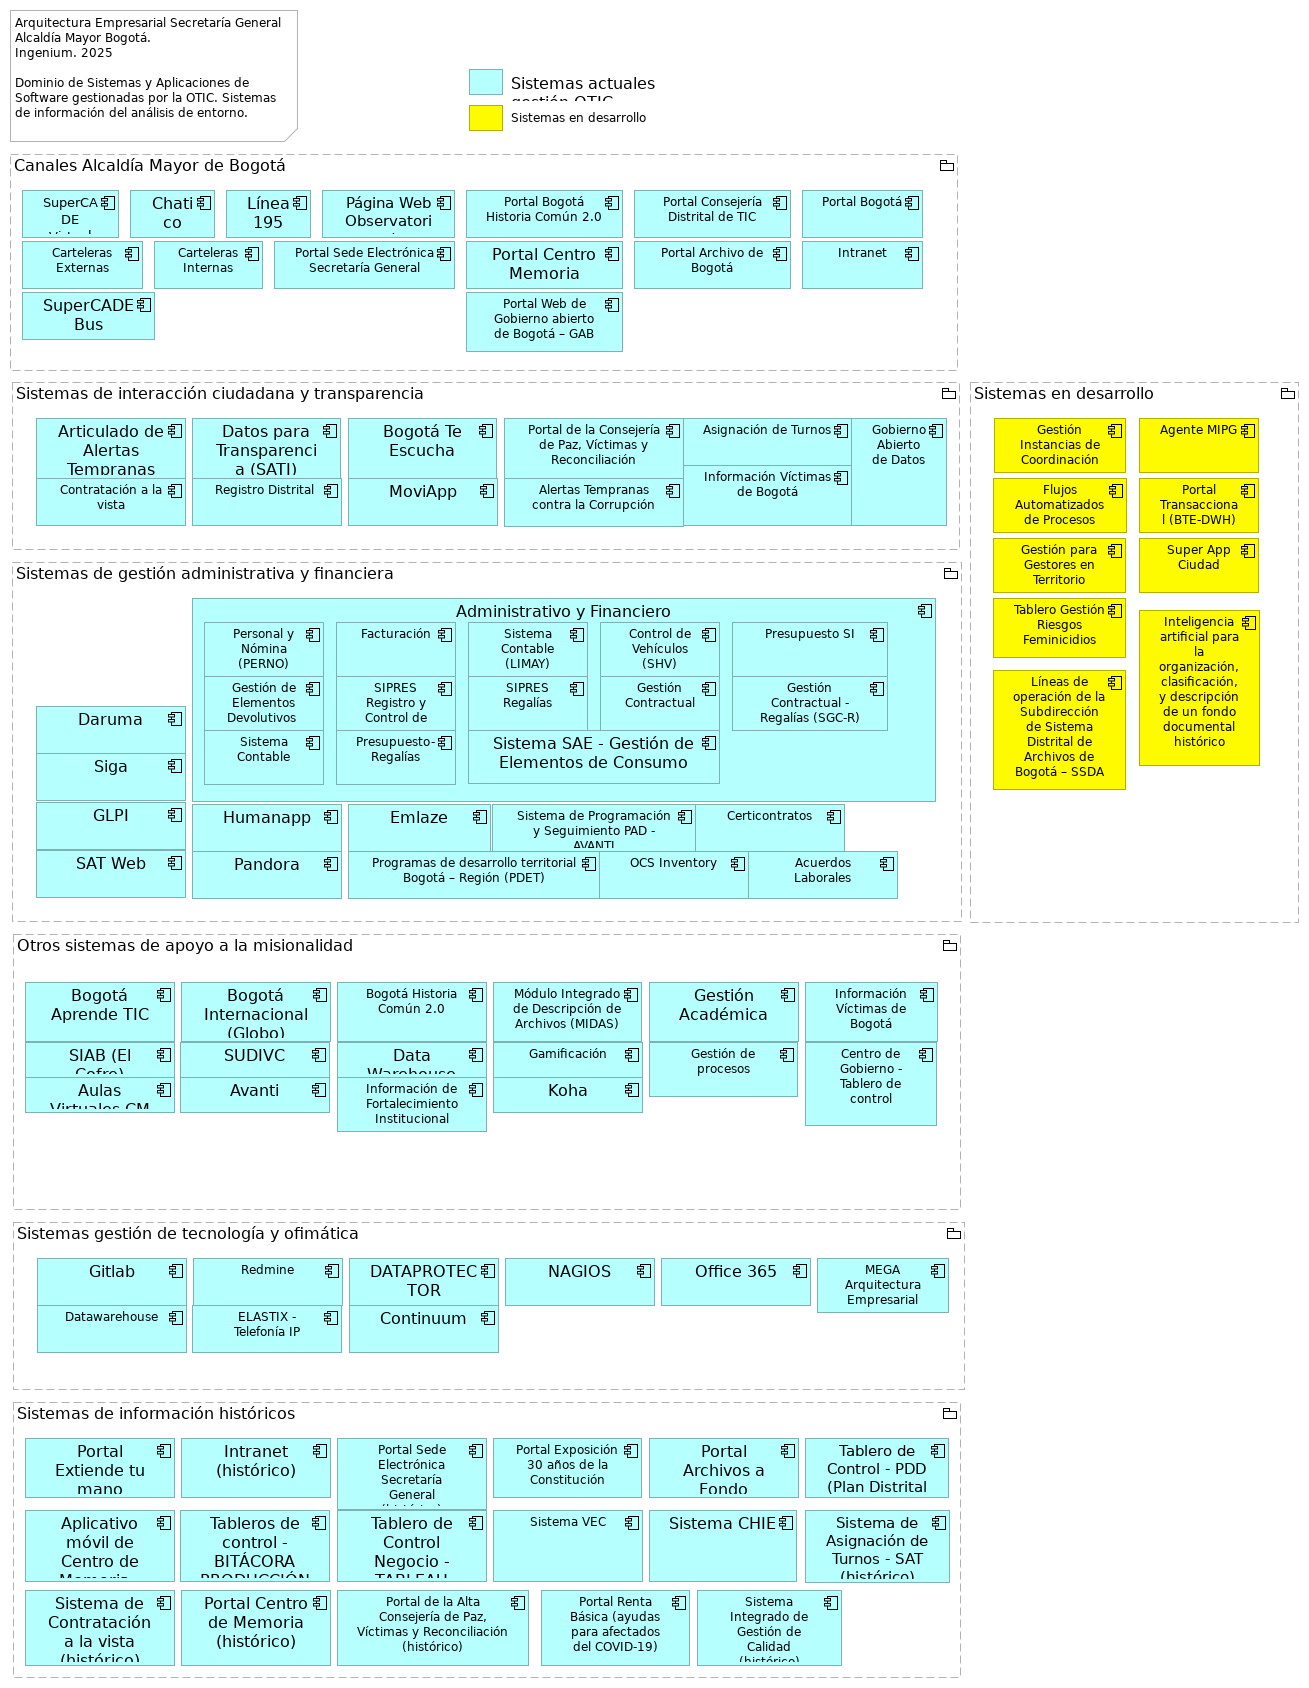
\includegraphics{images/06.2n2.1a.SIdelAnalisisdeEntorno.png}
\caption{06.2n2.1a. SI del Analisis de Entorno. \emph{Fuente:
Elaboración propia con información del equipo servicios tecnológicos de
la OTIC}}\label{fig:id-097745511d984e7eaf02b5ad5a93e7a8}
\end{figure}

\subsubsection{Elementos del Modelo}\label{sec:elementos-del-modelo}

\begin{longtable}[]{@{}
  >{\raggedright\arraybackslash}p{(\columnwidth - 4\tabcolsep) * \real{0.3000}}
  >{\raggedright\arraybackslash}p{(\columnwidth - 4\tabcolsep) * \real{0.2000}}
  >{\raggedright\arraybackslash}p{(\columnwidth - 4\tabcolsep) * \real{0.5000}}@{}}
\caption{\label{tbl:tblelement-06.2n2.1a.SIdelAnalisisdeEntorno-id}Elementos
de la vista.}\tabularnewline
\toprule\noalign{}
\begin{minipage}[b]{\linewidth}\raggedright
Nombre
\end{minipage} & \begin{minipage}[b]{\linewidth}\raggedright
Tipo
\end{minipage} & \begin{minipage}[b]{\linewidth}\raggedright
Documentación
\end{minipage} \\
\midrule\noalign{}
\endfirsthead
\toprule\noalign{}
\begin{minipage}[b]{\linewidth}\raggedright
Nombre
\end{minipage} & \begin{minipage}[b]{\linewidth}\raggedright
Tipo
\end{minipage} & \begin{minipage}[b]{\linewidth}\raggedright
Documentación
\end{minipage} \\
\midrule\noalign{}
\endhead
\bottomrule\noalign{}
\endlastfoot
Portales Institucionales y de Contenido & Grouping & \\
Portal Bogotá Historia Común 2.0 & Application Component & Portal para
mostrar infografías de Bogotá. La ciudadanía provee historias cotidianas
de su localidad y un grupo de análisis del Archivo de Bogotá determina
la pertinencia para su publicación. Sección del Portal de Archivo de
Bogotá. \\
Portal Bogotá Capital Digital & Application Component & Plataforma
unificada creada por la~Secretaría General de la Alcaldía Mayor de
Bogotá~para facilitar el acceso de la ciudadanía a más de~1.400 trámites
y servicios en línea. \\
& & \\
Portal Consejería Distrital de TIC & Application Component & Sitio web
institucional de la Alta Consejería Distrital de TIC. \\
Portal Centro Memoria & Application Component & Herramienta de
información para el fomento de la cultura y los derechos humanos.
Publica experiencias vividas para las víctimas del conflicto armado en
Colombia. Sitio http://centromemoria.gov.co. \\
& & \\
Portal Archivo de Bogotá & Application Component & Sitio web
institucional del Archivo de Bogotá. \\
Portal Bogotá & Application Component & Portal de la Alcaldía Mayor de
Bogotá orientado a la publicación de la Gestión del alcalde, noticias de
entidades y noticias de las localidades. \\
& & \\
Sistemas en Desarrollo & Grouping & \\
Gestión Instancias de Coordinación & Application Component & Componente
de aplicación para facilitar la interacción y el acercamiento
(realimentación) de los ciudadanos. \\
& & \\
Agente MIPG & Application Component & Componente de aplicación para
facilitar la interacción y el acercamiento (realimentación) de los
ciudadanos. \\
& & \\
Flujos Automatizados de Procesos Empleado con TH y Contratistas &
Application Component & Componente de aplicación para facilitar la
interacción y el acercamiento (realimentación) de los ciudadanos. \\
& & \\
Portal Transaccional & Application Component & Componente de aplicación
para facilitar la interacción y el acercamiento (realimentación) de los
ciudadanos. \\
& & \\
Gestión para Gestores en Territorio & Application Component & Componente
de aplicación para facilitar la interacción y el acercamiento
(realimentación) de los ciudadanos. \\
& & \\
Super App Ciudad & Application Component & Componente de aplicación para
facilitar la interacción y el acercamiento (realimentación) de los
ciudadanos. \\
& & \\
Tablero Gestión Riesgos Feminicidios & Application Component &
Componente de aplicación para facilitar la interacción y el acercamiento
(realimentación) de los ciudadanos. \\
& & \\
Canales Alcaldía Mayor de Bogotá & Grouping & \\
SuperCADE Virtual & Application Component & Plataforma digital
desarrollada por la~Secretaría General de la Alcaldía Mayor de
Bogotá~que permite a la ciudadanía acceder de manera rápida y segura a
más de 200 trámites y servicios en línea, sin necesidad de desplazarse
físicamente.~ \\
& & \\
Chatico & Application Component & Agente virtual basado en inteligencia
artificial que facilita el acceso de la ciudadanía a información sobre
trámites, servicios, ayudas distritales y participación ciudadana.
Chatico está disponible a través de la página web oficial y por WhatsApp
(+57 316 0231524). \\
& & \\
Línea 195 & Application Component & Canal telefónico oficial de atención
ciudadana operado por la~Secretaría General de la Alcaldía Mayor de
Bogotá, creado para ofrecer información clara, veraz y oportuna sobre
trámites, servicios, campañas y entidades del Distrito Capital. \\
& & \\
Página Web Observatorio de Víctimas del conflicto Armado & Application
Component & Conflicto armado de Bogotá D.C. reportadas por la Oficina
Consejería Distrital de Paz, Victimas y Reconciliacion \\
Carteleras Externas & Application Component & Portales de visualización
pública a la ciudadanía en los sitios de atención. \\
Carteleras Internas & Application Component & Portales de visualización
pública a los funcionarios y contratistas de la Secretaría General. \\
Gestión Contractual - Regalías (SGC-R) & Application Component & Sistema
de Gestión Contractual, módulo de regalías \\
Portal Sede Electrónica Secretaría General & Application Component &
Sitio web oficial de la Secretaría General. Se publica información
pública y en cumplimiento de obligaciones legales. \\
Sistemas de interacción ciudadana y transparencia & Grouping & \\
Articulado de Alertas Tempranas (SAAT) & Application Component & Sistema
de apoyo a la estrategia de la Secretaría Distrital de la Mujer (ley Ley
248 de 1995 y Ley 1257 de 2008): identificación del riesgo posible
víctima, gestión del riesgo y reducción del riesgo. \\
& & \\
Datos para Transparencia (SATI) & Application Component & Sistema de
tableros de control con datos relevantes, actualizados y comprensibles,
incluyendo alertas tempranas contra la corrupción para facilitar la
interacción y el acercamiento (realimentación) de los ciudadanos.
Plataforma que facilita el acceso a datos e información gubernamental.
Soporta el proceso de Gobierno abierto y relacionamiento con la
ciudadanía. \\
& & \\
Bogotá Te Escucha & Application Component & Sistema para el registro de
peticiones, quejas y sugerencias de la ciudadanía \\
Portal de la Consejería de Paz, Víctimas y Reconciliación & Application
Component & Portal donde se publican noticias y eventos relacionados con
la misionalidad de la Consejería de Paz, Víctimas y Reconciliación. \\
Asignación de Turnos & Application Component & Sistema de Asignación de
Turnos en los puntos de atención de la ciudad (Cades, Súper Cades,
puntos de encuentro) \\
Gobierno Abierto de Datos & Application Component & Portal para la
publicación de datos abiertos de Distrito con el fin de ser consultados
por la Ciudadanía y utilizados en toma de decisiones o análisis de
información \\
Información Víctimas de Bogotá & Application Component & Módulo
Integrado de Reportes del Sistema. Sistema de Información de Víctimas de
Bogotá - Para registrar la gestión de atención integral a las víctimas.
Sistema que utiliza el operador externo para realizar entregas de Ayuda
Humanitaria Inmediata. \\
Contratación a la vista & Application Component & Sistema de registro de
contratos distritales \\
Registro Distrital & Application Component & Se publican todos los actos
administrativos del Distrito, de cara al ciudadano. \\
MoviApp & Application Component & Aplicativo que permite el uso el
registro del uso en bicicleta por parte de los funcionarios de las
entidades del distrito. \\
Alertas Tempranas contra la Corrupción & Application Component & Sistema
Alertas Tempranas contra la Corrupción \\
Sistemas de gestión administrativa y financiera & Grouping & \\
Administrativo y Financiero & Application Component & Grupo de sistema
de soporte a la gestión financiera, gestión de servicios
administrativos, tecnológicos, y gestión de recursos físicos. \\
& & \\
Personal y Nómina (PERNO) & Application Component & Módulo de Personal y
Nómina (PERNO, heredado de SICAPITAL. \\
& & \\
Facturación & Application Component & Sistema de Facturación de la
Subdirección de Servicio a la Ciudadanía \\
Sistema Contable (LIMAY) & Application Component & LIMAY, heredado de
SICAPITAL. Sistema contable que maneja el libro mayor de la entidad. \\
& & \\
Control de Vehículos (SHV) & Application Component & Sistema de control
de vehículos \\
Presupuesto SI & Application Component & Sistema presupuestal de la
Entidad \\
Gestión de Elementos Devolutivos & Application Component & Sistema
control de gestión de elementos devolutivos (SAI, heredado de
SICAPITAL). \\
& & \\
SIPRES Registro y Control de Presupuesto & Application Component &
Registro y control de la información de presupuesto de la Secretaría
General (SIPRES). \\
& & \\
SIPRES Regalías & Application Component & Sistema para manejo y control
del presupuesto de regalías (SIPRES REGALIAS). \\
& & \\
Gestión Contractual & Application Component & Sistema de Gestión
Contractual \\
Gestión Contractual - Regalías (SGC-R) & Application Component & Sistema
de Gestión Contractual, módulo de regalías \\
Sistema Contable & Application Component & Sistema contable maneja el
libro mayor de la entidad. \\
Presupuesto-Regalías & Application Component & Sistema SIPRES - de
Presupuesto - Regalías \\
Daruma & Application Component & Sistema institucional de gestión de la
calidad utilizado por la Secretaría General para centralizar,
automatizar y hacer seguimiento a procesos clave como la administración
de documentos, indicadores, auditorías y acciones de mejora. \\
& & \\
Siga & Application Component & Sistema Integrado de Gestión Documental,
Archivo y Correspondencia para gesttión de todas la comunicaciones
internas de la SG (Memorandos, Circulares, etc), externas y algunas
interoperabilidades. \\
& & \\
GLPI & Application Component & Sistema de soporta a la gestión de
servicios administrativos y tecnológicos, donde se registran y gestionan
las solicitudes de servicios TIC de diferentes categorías de la
Secretaría General. Mesa de ayuda (Gestión de solicitudes de atención
ante incidentes tecnológicos). \\
& & \\
Humanapp & Application Component & Aplicativo de uso interno de la
Secretaría General para generar desprendibles de pago para funcionarios
y certificaciones laborales, de seguridad social y de ingresos y
retenciones. Utiliza una vista del sistema PERNO. Apoya la gestión del
talento humano. Aplicativo de generación de desprendibles de pago para
funcionarios y certificaciones laborales, de seguridad social y de
ingresos y retenciones. \\
& & \\
Emlaze & Application Component & Sistema para la planeación de recursos
empresariales (ERP) de la Imprenta Distrital y control de ejecución y
consumo de insumos en el ejercicio de imprenta. \\
& & \\
Sistema de Programación y Seguimiento PAD - AVANTI & Application
Component & Sistema de Información para registrar avance de programación
y seguimiento de metas plan de desarrollo de la estidades distritales
SDARIV relacionadas con atención integral a las víctimas. \\
Certicontratos & Application Component & Sitio privado interno donde se
muestran los contratos de la entidad, ejecutados desde 2015. \\
SAT Web & Application Component & Sistema de Asignación de Turnos en los
puntos de atención a la ciudadanía (Red Cade). \\
& & \\
Pandora & Application Component & Implementación de temas precontractual
y planeación. \\
& & \\
Programas de desarrollo territorial Bogotá -- Región (PDET) &
Application Component & Plataforma tecnológica para habilitar los
procesos participativos de construcción de paz, con énfasis en la
formulación de los programas de desarrollo territorial Bogotá -- Región
(PDET -- BR). \\
OCS Inventory & Application Component & Sistema para gestionar
información del inventario de los componentes lógicos de los elementos
ofimáticos \\
Acuerdos Laborales & Application Component & Sistema de Información de
Acuerdos Laborales - Registro de los acuerdos laborales entre la SG y
los sindicatos del Distrito \\
Sistemas de fortalecimiento de capacidades, del conocimiento y datos
para la gestión pública & Grouping & \\
Bogotá Aprende TIC & Application Component & Portal de apoya los
procesos de Gobierno abierto y relacionamiento con la ciudadanía, y
Fortalecimiento de la Gestión Pública. \\
& & \\
Bogotá Internacional (Globo) & Application Component & Registro de
acciones de cooperación internacional. Utilizado en el proceso de
Fortalecimiento de la Gestión Pública. \\
& & \\
Bogotá Historia Común 2.0 & Application Component & Sistema para mostrar
infografías de Bogotá. La ciudadanía provee historias cotidianas de su
localidad y un grupo de análisis del Archivo de Bogotá determina la
pertinencia para su publicación.. \\
Módulo Integrado de Descripción de Archivos (MIDAS) & Application
Component & Catalogación y descripción de algunos registros del Archivo
de Bogotá \\
Gestión Académica & Application Component & Moodle para capacitación de
servidores de la SG en diferentes temas \\
MEGA Arquitectura Empresarial & Application Component & Herramienta de
Arquitectura Empresarial enfocada a los resultados de negocios ayuda a
las empresas a gestionar la innovación e iniciativas estratégicas
(también llamado MEGA). \\
& & \\
SIAB (El Cofre) & Application Component & Sistema de Información del
Archivo de Bogotá SIAB. Registro del acervo documental de Bogotá
(documentos históricos, planos, mapas, transferencias bibliograficas,
entre otros). Permite automatizar los procesos archivísticos y técnicos
que realiza el Archivo, tales como llevar un registro de los Ingresos
Documentales (antes área de acopio), para la descripción y catalogación
de la documentación, propios del proceso de Gestión de la Función
Archivística y del Patrimonio Documental, para su custodia y
conservación permanente. Utilizado en los procesos de Gobierno abierto y
relacionamiento con la ciudadanía, y Fortalecimiento de la Gestión
Pública. \\
& & \\
SUDIVC & Application Component & Sistema Unificado Distrital de
Inspección, Vigilancia y Control -- SUDIVC. \\
& & \\
Data Warehouse & Application Component & Almacenes de datos de trabajo
de SG. Bodega de datos con diversas fuentes de información para el
análisis y transformación de datos de interés. \\
& & \\
Gamificación & Application Component & Herramienta web para el
autoaprendizaje y refuerzo temático para cualificación a servidores
públicos \\
Bogotá Global & Application Component & Sistema donde se registran las
acciones de Cooperación Internacional de Bogotá con otras ciudades e
instituciones del mundo \\
Koha & Application Component & Sistema Integrado de Gestión de
Bibliotecas. Relacionado con la Gestión del conocimiento. \\
& & \\
SIVIC & Application Component & Sistema de Información de Víctimas de
Bogotá para registrar la gestión de atención integral a las víctimas.
Interviene en los procesos de Paz, víctimas y reconciliación, y
Fortalecimiento de la Gestión Pública. Interviene en los procesos de
Paz, víctimas y reconciliación, y Fortalecimiento de la Gestión
Pública. \\
& & \\
Avanti & Application Component & Sistema de Información para registrar
avance de programación y seguimiento de metas plan de desarrollo de las
entidades distritales SDARIV relacionadas con atención integral a las
víctimas. \\
& & \\
Información de Fortalecimiento Institucional & Application Component &
Sistema de Información de Fortalecimiento Institucional \\
Sistema Integrado de Gestión & Application Component & Sistema Integrado
de Gestión de Calidad- Histórico \\
Gestión de procesos & Application Component & Sistema de Gestión de
procesos \\
Sistemas de desarrollo de software & Grouping & \\
Gitlab & Application Component & Plataforma de desarrollo de software y
colaboración. \\
& & \\
Redmine & Application Component & Sistema de documentación técnica de
los Sistemas de Información. Portales Web y Aplicativos de la SG \\
Datawarehouse & Application Component & Bodega de datos con varias
fuentes - Analítica de datos \\
Ofimática y colaboración & Grouping & \\
Office 365 & Application Component & Herramientas de ofimática y
colaboración SG. \\
& & \\
\end{longtable}

\subsection{Alineación de aplicaciones de software con los procesos
SG}\label{sec:alineaciuxf3n-de-aplicaciones-de-software-con-los-procesos-sg}

\begin{quote}
\end{quote}

Secretaria General Alcaldía Mayor de Bogotá (SG) cuenta con sistemas de
información que soportan las actividades gestionadas por los procesos
institucionales: misionales, estratégicos, de apoyo y de evaluación y
control. Del análisis de las fuentes y el levantamientos de información
presentamos la alineación de las aplicaciones de software de SG, con los
procesos de negocio y el estado actual de cada una.

\begin{longtable}[]{@{}
  >{\raggedright\arraybackslash}p{(\columnwidth - 4\tabcolsep) * \real{0.2045}}
  >{\raggedright\arraybackslash}p{(\columnwidth - 4\tabcolsep) * \real{0.2992}}
  >{\raggedright\arraybackslash}p{(\columnwidth - 4\tabcolsep) * \real{0.4962}}@{}}
\caption{\label{tbl:tblelement-vision.entregables-id}Aplicaciones y
Procesos del dominio de sistemas de información de la
SG.}\tabularnewline
\toprule\noalign{}
\begin{minipage}[b]{\linewidth}\raggedright
Proceso
\end{minipage} & \begin{minipage}[b]{\linewidth}\raggedright
Sistema de Información
\end{minipage} & \begin{minipage}[b]{\linewidth}\raggedright
Oportunidad de Mejora
\end{minipage} \\
\midrule\noalign{}
\endfirsthead
\toprule\noalign{}
\begin{minipage}[b]{\linewidth}\raggedright
Proceso
\end{minipage} & \begin{minipage}[b]{\linewidth}\raggedright
Sistema de Información
\end{minipage} & \begin{minipage}[b]{\linewidth}\raggedright
Oportunidad de Mejora
\end{minipage} \\
\midrule\noalign{}
\endhead
\bottomrule\noalign{}
\endlastfoot
Control Disciplinario & Gestión Documental - SIGA & Actualización de la
versión de la aplicación y su infraestructura \\
Evaluación del Sistema de Control Interno & Gestión Documental - SIGA &
Actualización de la versión de la aplicación y su infraestructura \\
Gestión Jurídica & Gestión Documental - SIGA & Actualización de la
versión de la aplicación y su infraestructura \\
Gestión de contratación & Administrativo y Financiero (Gestión
Contractual) & Actualización tecnológica para optimizar el rendimiento y
acceso al sistema de información y atención de requerimientos a
demanda \\
Gestión Financiera & Administrativo y Financiero (Facturación, LIMAY,
Gestión Contractual, SIPRES) & Actualización tecnológica para optimizar
el rendimiento y acceso al sistema de información y atención de
requerimientos a demanda \\
Gestión de servicios administrativos y tecnológicos & GitLab, GLPI &
Atención de requerimientos a demanda \\
Gestión de servicios administrativos y tecnológicos & Administrativo y
Financiero (Inventario, SAI, SAE, Control de vehículos) & Actualización
tecnológica para optimizar el rendimiento y acceso al sistema de
información y atención de requerimientos a demanda \\
Gestión de recursos físicos & Administrativo y Financiero (Inventario,
SAI SAE, Control de vehículos) & Actualización tecnológica para
optimizar el rendimiento y acceso al sistema de información y atención
de requerimientos a demanda \\
Gestión del Talento Humano & Administrativo y Financiero (PERNO) &
Actualización tecnológica para optimizar el rendimiento y acceso al
sistema de información y atención de requerimientos a demanda \\
Gestión del Talento Humano & HUMANAPP & Actualización tecnológica para
optimizar el rendimiento y acceso al sistema de información y atención
de requerimientos a demanda \\
Gobierno abierto y relacionamiento con la ciudadanía & Bogotá Te Escucha
& Actualización de la versión de la aplicación y su infraestructura \\
Gobierno abierto y relacionamiento con la ciudadanía & Data Warehouse &
Vincular más Fuentes de información \\
Gobierno abierto y relacionamiento con la ciudadanía & SAT Web &
Actualización de su infraestructura \\
Gobierno abierto y relacionamiento con la ciudadanía & SUDIVC & Atención
de requerimientos a demanda \\
Paz, víctimas y reconciliación & SIVIC & Atención de requerimientos a
demanda \\
Paz, víctimas y reconciliación & AVANTI & Atención de requerimientos a
demanda \\
Fortalecimiento de la Gestión Pública & SIAB (Cofre) & Atención de
requerimientos a demanda \\
Fortalecimiento de la Gestión Pública & KOHA & Atención de
requerimientos a demanda \\
Fortalecimiento de la Gestión Pública & Datos para la transparencia
(SATI) & Atención de requerimientos a demanda \\
Fortalecimiento de la Gestión Pública & EMLAZE & Atención de
requerimientos a demanda y con proveedor externo para el caso de
Emlaze \\
Direccionamiento Estratégico & DARUMA & Atención de requerimientos a
demanda con proveedor externo \\
Gestión estratégica de comunicación e información & Gestión Documental -
SIGA & Actualización de la versión de la aplicación y su
infraestructura \\
Fortalecimiento Institucional & Gestión académica & Atención de
requerimientos a demanda \\
Gestión de alianzas e internacionalización de Bogotá & Globo & Atención
de requerimientos a demanda \\
Gestión del conocimiento & Bogotá Aprende TIC & Atención de
requerimientos a demanda \\
\end{longtable}

Es importante destacar que el sistema Integrado de Gestión de Calidad
DARUMA, el Sistema de Gestión de Incidentes y Solicitudes GLPI, y el
Sistema de Gestión Documental SIGA, son sistemas transversales que
soportan todos los procesos de la Secretaría General de la Alcaldía
Mayor de Bogotá D.C.

\begin{figure}
\centering
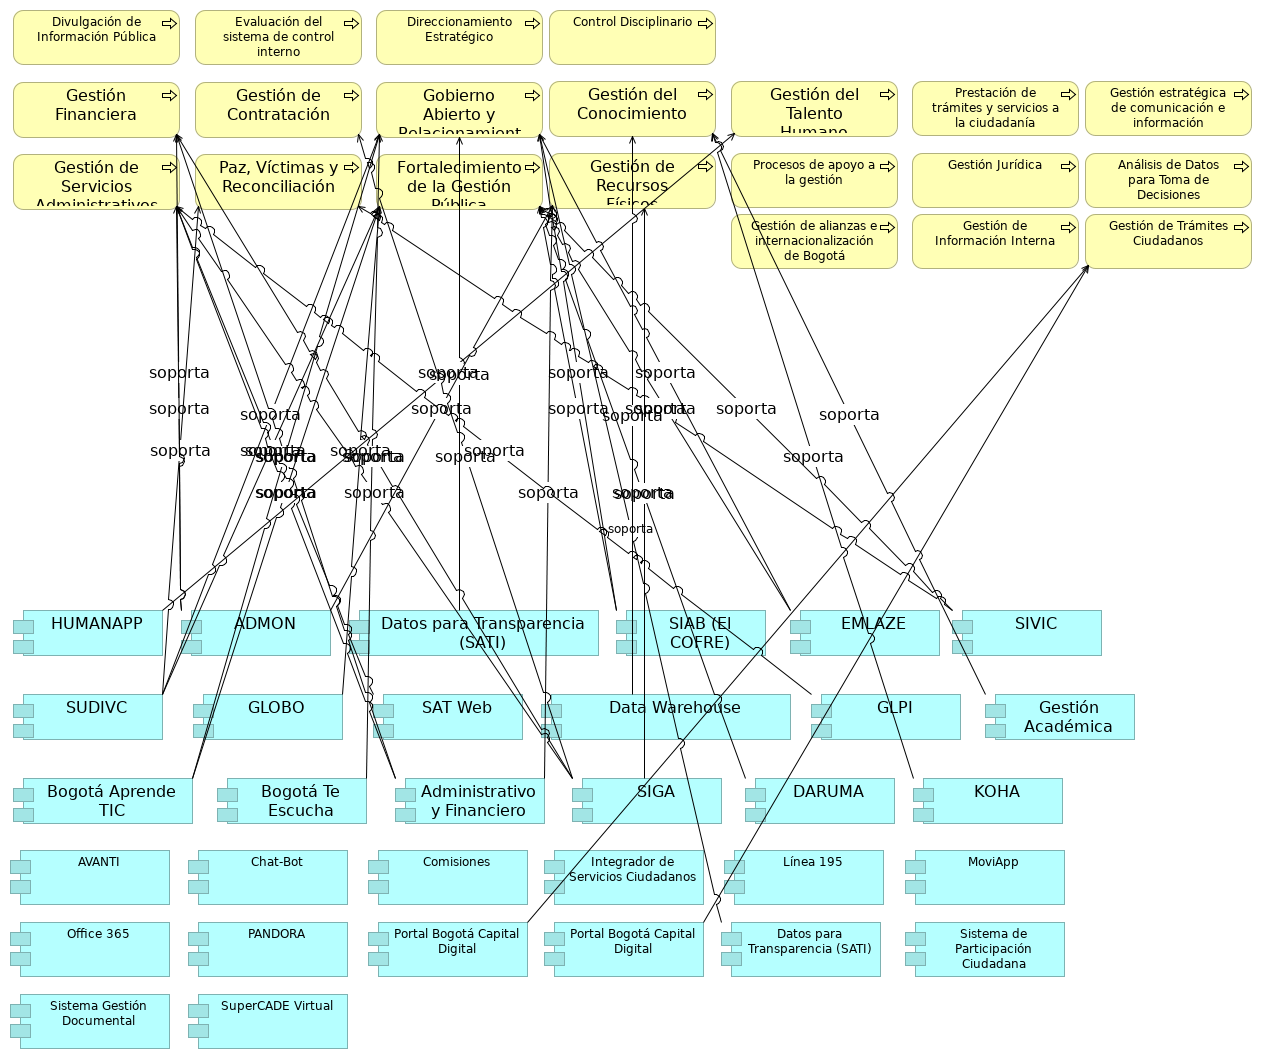
\includegraphics{images/06.2n3.a.AplicacionesyProcesos.png}
\caption{06.2n3.a. Aplicaciones y Procesos. \emph{Fuente: Elaboración
propia con información del equipo servicios tecnológicos de la
OTIC}}\label{fig:id-7812cd6a3a0d4d5783b00f16f2c5826b}
\end{figure}

\subsubsection{Elementos del Modelo}\label{sec:elementos-del-modelo-1}

\begin{longtable}[]{@{}
  >{\raggedright\arraybackslash}p{(\columnwidth - 4\tabcolsep) * \real{0.3000}}
  >{\raggedright\arraybackslash}p{(\columnwidth - 4\tabcolsep) * \real{0.2000}}
  >{\raggedright\arraybackslash}p{(\columnwidth - 4\tabcolsep) * \real{0.5000}}@{}}
\caption{\label{tbl:tblelement-06.2n3.a.AplicacionesyProcesos-id}Elementos
de la vista.}\tabularnewline
\toprule\noalign{}
\begin{minipage}[b]{\linewidth}\raggedright
Nombre
\end{minipage} & \begin{minipage}[b]{\linewidth}\raggedright
Tipo
\end{minipage} & \begin{minipage}[b]{\linewidth}\raggedright
Documentación
\end{minipage} \\
\midrule\noalign{}
\endfirsthead
\toprule\noalign{}
\begin{minipage}[b]{\linewidth}\raggedright
Nombre
\end{minipage} & \begin{minipage}[b]{\linewidth}\raggedright
Tipo
\end{minipage} & \begin{minipage}[b]{\linewidth}\raggedright
Documentación
\end{minipage} \\
\midrule\noalign{}
\endhead
\bottomrule\noalign{}
\endlastfoot
Divulgación de Información Pública & Business Process & Proceso de
negocio para la difusión optimizada de información a través de sistemas
digitales. \\
& & \\
Evaluación del sistema de control interno & Business Process & Evaluar
de manera independiente y objetiva el Sistema de Control Interno de la
Secretaría General de la Alcaldía Mayor de Bogotá, mediante la
realización de auditorías internas de gestión, seguimientos e informes
regulatorios programados en el Plan de Anual de Auditorías, y la
atención a organismos de control, con el propósito de contribuir al
mejoramiento continuo de la gestión institucional. \\
& & \\
Direccionamiento Estratégico & Business Process & Formular, implementar,
hacer monitoreo y seguimiento a las políticas públicas competencia de la
Secretaría General, a los planes institucionales, a los proyectos de
inversión, y gestionar el presupuesto de inversión mediante la
definición de orientaciones, metodologías, la retroalimentación,
acompañamiento y articulación a las dependencias de la entidad con el
fin de cumplir el logro de la misión y los objetivos institucionales, en
el marco de una cultura de transparencia. \\
& & \\
Control Disciplinario & Business Process & Adelantar los procesos
disciplinarios contra los(as) servidores(as) y exservidores(as) de la
Secretaría General de la Alcaldía Mayor de Bogotá D.C., y prevenir las
conductas disciplinarias mediante la aplicación de las normas vigentes
en materia disciplinaria y el desarrollo de la estrategia preventiva con
el fin determinar la posible responsabilidad disciplinaria, y evitar la
ocurrencia de faltas disciplinarias por parte de estos. \\
& & \\
Gestión del Conocimiento & Business Process & Gestionar el conocimiento
y la innovación de la Secretaría General de la Alcaldía Mayor de Bogotá,
mediante la identificación, generación, sistematización, análisis,
transferencia y conservación del conocimiento estratégico y la promoción
de la innovación, con el fin de fortalecer el aprendizaje, el
mejoramiento organizacional y la toma de decisiones basada en
evidencias. \\
& & \\
Gestión del Talento Humano & Business Process & Gestionar el capital
humano de la Secretaría General, y vincular y administrar el Gabinete
distrital y jefatura del talento humano interno mediante el Plan
Estratégico de Talento Humano para la Secretaría General y el trámite de
situaciones administrativas con el fin de fortalecer el sentido de
pertenencia y contribuir a la calidad de vida del talento humano de la
entidad. \\
& & \\
Prestación de trámites y servicios a la ciudadanía & Business Process &
Proceso central para la interacción con los ciudadanos. \\
& & \\
Gestión estratégica de comunicación e información & Business Process &
Mantener informados a los distintos grupos de valor e interés acerca de
los programas, proyectos y gestión de la Administración Distrital a
través de la formulación y la implementación de estrategias de
comunicación pública con el propósito de interactuar y mantener la
confianza por parte de la entidad y de la ciudadanía en general. \\
& & \\
Gestión Financiera & Business Process & Gestionar las operaciones
financieras con cargo al presupuesto asignado a la entidad, a través del
registro de las operaciones económicas en contabilidad para garantizar
la elaboración y reporte de los estados financieros a los entes de
control en forma comprensible, relevante y confiable, para que sean
consultados por los ciudadanos y por los interesados en la información
financiera. \\
& & \\
Gestión de Contratación & Business Process & Gestionar la contratación
de bienes, servicios y obras, mediante el desarrollo de procesos
contractuales transparentes y conforme a la normativa legal vigente para
satisfacer las necesidades de contratación de las dependencias de la
Secretaría General de la Alcaldía Mayor de Bogotá, y contribuir al
cumplimento de sus metas y objetivos. \\
& & \\
Gobierno Abierto y Relacionamiento con la Ciudadanía & Business Process
& Fortalecer relación entre la administración distrital y la ciudadanía
mediante la formulación de lineamientos, desarrollo de estrategias y
proyectos, fortalecimiento de capacidades, seguimiento y evaluación en
materia de servicio a la ciudadanía, gobierno abierto y transformación
digital de la Secretaría General y de las entidades distritales, para el
acceso oportuno, efectivo y de calidad a la oferta institucional de
bienes y servicios. \\
& & \\
Gestión de Recursos Físicos & Business Process & Administrar los bienes
que legalmente están a cargo de la Secretaría General de la Alcaldía
Mayor de Bogotá D.C. mediante su recepción, asignación, mantenimiento,
control, baja y/o destinación final con el fin de cubrir las necesidades
de recursos físicos de las dependencias. \\
& & \\
Procesos de apoyo a la gestión & Business Process & Procesos internos
que facilitan la operación de la entidad. \\
& & \\
Gestión Jurídica & Business Process & Asesorar y representar
jurídicamente a la Secretaría General de la Alcaldía Mayor Bogotá D.C.
mediante el análisis, trámite, defensa, solución y respuesta de asuntos
de carácter jurídico que surjan en el desarrollo de las funciones de
acuerdo con la normatividad vigente. \\
& & \\
Análisis de Datos para Toma de Decisiones & Business Process & Proceso
de negocio que utiliza software especializado para el análisis de
datos. \\
& & \\
Gestión de Servicios Administrativos y Tecnológicos & Business Process &
Apoyar la gestión de la Entidad a través de la prestación de los
servicios administrativos y tecnológicos, así como, de la gestión
documental, con el fin de satisfacer las necesidades de las dependencias
en la materia, al igual que conservar y preservar la memoria
institucional. \\
& & \\
Paz, Víctimas y Reconciliación & Business Process & Gestionar políticas,
programas y estrategias dirigidas a las víctimas, población en proceso
de reintegración, reincorporación, comparecientes de fuerza pública y
ciudadanía en general por medio de la asistencia, atención, reparación,
y acciones de memoria, reconciliación y construcción de paz territorial
con el propósito de que Bogotá sea un territorio de paz y
reconciliación, donde todos puedan volver a empezar. \\
& & \\
Fortalecimiento de la Gestión Pública & Business Process & Generar
capacidades institucionales en las entidades distritales a través del
desarrollo de estudios, investigaciones y estrategias relacionadas con
el fortalecimiento de la gestión, impresión de artes gráficas y la
publicación de la Gaceta Pública en el registro distrital; con el fin,
de modernizar y mejorar el desempeño de la administración distrital. \\
& & \\
Gestión de alianzas e internacionalización de Bogotá & Business Process
& Facilitar acciones estratégicas de cooperación, relacionamiento y
posicionamiento internacional, mediante la gestión de interacciones con
actores nacionales e internacionales, con el fin de movilizar recursos
técnicos y financieros, generar alianzas estratégicas y posicionar a
Bogotá como un referente global. De esta manera, se contribuirá a la
implementación del Plan de Desarrollo Distrital, fortalecerá las
políticas públicas y la gestión del Distrito, y se alineará con
iniciativas globales como la Agenda 2030. \\
& & \\
Gestión de Información Interna & Business Process & Proceso de
recolección, procesamiento y distribución de información dentro de la
entidad. \\
& & \\
Gestión de Trámites Ciudadanos & Business Process & Proceso de atención
y resolución de solicitudes y gestiones de los ciudadanos. \\
& & \\
Humanapp & Application Component & Aplicativo de uso interno de la
Secretaría General para generar desprendibles de pago para funcionarios
y certificaciones laborales, de seguridad social y de ingresos y
retenciones. Utiliza una vista del sistema PERNO. Apoya la gestión del
talento humano. Aplicativo de generación de desprendibles de pago para
funcionarios y certificaciones laborales, de seguridad social y de
ingresos y retenciones. \\
& & \\
ADMON & Application Component & Se relaciona con la gestión financiera,
gestión de servicios administrativos y tecnológicos, y gestión de
recursos físicos. \\
& & \\
Datos para Transparencia (SATI) & Application Component & Sistema de
tableros de control con datos relevantes, actualizados y comprensibles,
incluyendo alertas tempranas contra la corrupción para facilitar la
interacción y el acercamiento (realimentación) de los ciudadanos.
Plataforma que facilita el acceso a datos e información gubernamental.
Soporta el proceso de Gobierno abierto y relacionamiento con la
ciudadanía. \\
& & \\
SIAB (El Cofre) & Application Component & Sistema de Información del
Archivo de Bogotá SIAB. Registro del acervo documental de Bogotá
(documentos históricos, planos, mapas, transferencias bibliograficas,
entre otros). Permite automatizar los procesos archivísticos y técnicos
que realiza el Archivo, tales como llevar un registro de los Ingresos
Documentales (antes área de acopio), para la descripción y catalogación
de la documentación, propios del proceso de Gestión de la Función
Archivística y del Patrimonio Documental, para su custodia y
conservación permanente. Utilizado en los procesos de Gobierno abierto y
relacionamiento con la ciudadanía, y Fortalecimiento de la Gestión
Pública. \\
& & \\
Emlaze & Application Component & Sistema para la planeación de recursos
empresariales (ERP) de la Imprenta Distrital y control de ejecución y
consumo de insumos en el ejercicio de imprenta. \\
& & \\
SIVIC & Application Component & Sistema de Información de Víctimas de
Bogotá para registrar la gestión de atención integral a las víctimas.
Interviene en los procesos de Paz, víctimas y reconciliación, y
Fortalecimiento de la Gestión Pública. Interviene en los procesos de
Paz, víctimas y reconciliación, y Fortalecimiento de la Gestión
Pública. \\
& & \\
SUDIVC & Application Component & Sistema Unificado Distrital de
Inspección, Vigilancia y Control -- SUDIVC. \\
& & \\
Bogotá Internacional (Globo) & Application Component & Registro de
acciones de cooperación internacional. Utilizado en el proceso de
Fortalecimiento de la Gestión Pública. \\
& & \\
SAT Web & Application Component & Sistema de Asignación de Turnos en los
puntos de atención a la ciudadanía (Red Cade). \\
& & \\
Data Warehouse & Application Component & Almacenes de datos de trabajo
de SG. Bodega de datos con diversas fuentes de información para el
análisis y transformación de datos de interés. \\
& & \\
GLPI & Application Component & Sistema de soporta a la gestión de
servicios administrativos y tecnológicos, donde se registran y gestionan
las solicitudes de servicios TIC de diferentes categorías de la
Secretaría General. Mesa de ayuda (Gestión de solicitudes de atención
ante incidentes tecnológicos). \\
& & \\
Gestión Académica & Application Component & Moodle para capacitación de
servidores de la SG en diferentes temas \\
Bogotá Aprende TIC & Application Component & Portal de apoya los
procesos de Gobierno abierto y relacionamiento con la ciudadanía, y
Fortalecimiento de la Gestión Pública. \\
& & \\
Bogotá Te Escucha & Application Component & Sistema para el registro de
peticiones, quejas y sugerencias de la ciudadanía \\
Administrativo y Financiero & Application Component & Grupo de sistema
de soporte a la gestión financiera, gestión de servicios
administrativos, tecnológicos, y gestión de recursos físicos. \\
& & \\
Siga & Application Component & Sistema Integrado de Gestión Documental,
Archivo y Correspondencia para gesttión de todas la comunicaciones
internas de la SG (Memorandos, Circulares, etc), externas y algunas
interoperabilidades. \\
& & \\
Daruma & Application Component & Sistema institucional de gestión de la
calidad utilizado por la Secretaría General para centralizar,
automatizar y hacer seguimiento a procesos clave como la administración
de documentos, indicadores, auditorías y acciones de mejora. \\
& & \\
Koha & Application Component & Sistema Integrado de Gestión de
Bibliotecas. Relacionado con la Gestión del conocimiento. \\
& & \\
Avanti & Application Component & Sistema de Información para registrar
avance de programación y seguimiento de metas plan de desarrollo de las
entidades distritales SDARIV relacionadas con atención integral a las
víctimas. \\
& & \\
Chatico & Application Component & Agente virtual basado en inteligencia
artificial que facilita el acceso de la ciudadanía a información sobre
trámites, servicios, ayudas distritales y participación ciudadana.
Chatico está disponible a través de la página web oficial y por WhatsApp
(+57 316 0231524). \\
& & \\
Comisiones & Application Component & Sesión levantamiento no. 1. \\
& & \\
Integrador de Servicios Ciudadanos & Application Component & Plataforma
unificada para acceder a servicios y trámites ciudadanos. \\
& & \\
Línea 195 & Application Component & Canal telefónico oficial de atención
ciudadana operado por la~Secretaría General de la Alcaldía Mayor de
Bogotá, creado para ofrecer información clara, veraz y oportuna sobre
trámites, servicios, campañas y entidades del Distrito Capital. \\
& & \\
MoviApp & Application Component & Aplicativo que permite el uso el
registro del uso en bicicleta por parte de los funcionarios de las
entidades del distrito. \\
Office 365 & Application Component & Herramientas de ofimática y
colaboración SG. \\
& & \\
Pandora & Application Component & Implementación de temas precontractual
y planeación. \\
& & \\
Portal Bogotá Capital Digital & Application Component & Plataforma
unificada creada por la~Secretaría General de la Alcaldía Mayor de
Bogotá~para facilitar el acceso de la ciudadanía a más de~1.400 trámites
y servicios en línea. \\
& & \\
Portal Bogotá Capital Digital & Application Component & Plataforma
unificada creada por la~Secretaría General de la Alcaldía Mayor de
Bogotá~para facilitar el acceso de la ciudadanía a más de~1.400 trámites
y servicios en línea. \\
& & \\
Datos para Transparencia (SATI) & Application Component & Sistema de
tableros de control con datos relevantes, actualizados y comprensibles,
incluyendo alertas tempranas contra la corrupción para facilitar la
interacción y el acercamiento (realimentación) de los ciudadanos.
Plataforma que facilita el acceso a datos e información gubernamental.
Soporta el proceso de Gobierno abierto y relacionamiento con la
ciudadanía. \\
& & \\
Sistema de Participación Ciudadana & Application Component & Componente
de aplicación para facilitar la interacción y el acercamiento
(realimentación) de los ciudadanos. \\
& & \\
SuperCADE Virtual & Application Component & Plataforma digital
desarrollada por la~Secretaría General de la Alcaldía Mayor de
Bogotá~que permite a la ciudadanía acceder de manera rápida y segura a
más de 200 trámites y servicios en línea, sin necesidad de desplazarse
físicamente.~ \\
& & \\
\end{longtable}

undefined\#\# Relación Sistemas de Información Procesos

Presentamos la matriz de relación de los sistemas de información en
gestión de la Oficina de TI y los procesos institucionales de Secretaría
General. La matriz destacan aquellos sistemas que por su mayor nivel de
soporte a los procesos institucionales son transversales a la
Secretaría.

\begin{longtable}[]{@{}
  >{\raggedright\arraybackslash}p{(\columnwidth - 32\tabcolsep) * \real{0.0609}}
  >{\raggedright\arraybackslash}p{(\columnwidth - 32\tabcolsep) * \real{0.0389}}
  >{\raggedright\arraybackslash}p{(\columnwidth - 32\tabcolsep) * \real{0.0728}}
  >{\raggedright\arraybackslash}p{(\columnwidth - 32\tabcolsep) * \real{0.0305}}
  >{\raggedright\arraybackslash}p{(\columnwidth - 32\tabcolsep) * \real{0.0423}}
  >{\raggedright\arraybackslash}p{(\columnwidth - 32\tabcolsep) * \real{0.0338}}
  >{\raggedright\arraybackslash}p{(\columnwidth - 32\tabcolsep) * \real{0.0897}}
  >{\raggedright\arraybackslash}p{(\columnwidth - 32\tabcolsep) * \real{0.0491}}
  >{\raggedright\arraybackslash}p{(\columnwidth - 32\tabcolsep) * \real{0.0457}}
  >{\raggedright\arraybackslash}p{(\columnwidth - 32\tabcolsep) * \real{0.0914}}
  >{\raggedright\arraybackslash}p{(\columnwidth - 32\tabcolsep) * \real{0.0541}}
  >{\raggedright\arraybackslash}p{(\columnwidth - 32\tabcolsep) * \real{0.0660}}
  >{\raggedright\arraybackslash}p{(\columnwidth - 32\tabcolsep) * \real{0.0508}}
  >{\raggedright\arraybackslash}p{(\columnwidth - 32\tabcolsep) * \real{0.0863}}
  >{\raggedright\arraybackslash}p{(\columnwidth - 32\tabcolsep) * \real{0.0525}}
  >{\raggedright\arraybackslash}p{(\columnwidth - 32\tabcolsep) * \real{0.0914}}
  >{\raggedright\arraybackslash}p{(\columnwidth - 32\tabcolsep) * \real{0.0440}}@{}}
\caption{\label{tbl:tblelement-Relaciuxf3nSistemasProcesos-id}Relación
Sistemas de Información y Procesos de la SG. Fuente: información del
equipo servicios tecnológicos de la OTIC.}\tabularnewline
\toprule\noalign{}
\begin{minipage}[b]{\linewidth}\raggedright
Sistema o aplicación
\end{minipage} & \begin{minipage}[b]{\linewidth}\raggedright
Control Disciplinario
\end{minipage} & \begin{minipage}[b]{\linewidth}\raggedright
Evaluación del Sistema de Control Interno
\end{minipage} & \begin{minipage}[b]{\linewidth}\raggedright
Gestión Jurídica
\end{minipage} & \begin{minipage}[b]{\linewidth}\raggedright
Gestión de contratación
\end{minipage} & \begin{minipage}[b]{\linewidth}\raggedright
Gestión Financiera
\end{minipage} & \begin{minipage}[b]{\linewidth}\raggedright
Gestión de servicios administrativos y tecnológicos
\end{minipage} & \begin{minipage}[b]{\linewidth}\raggedright
Gestión de recursos físicos
\end{minipage} & \begin{minipage}[b]{\linewidth}\raggedright
Gestión de Talento Humano
\end{minipage} & \begin{minipage}[b]{\linewidth}\raggedright
Gobierno abierto y relacionamiento con la ciudadanía
\end{minipage} & \begin{minipage}[b]{\linewidth}\raggedright
Paz, víctimas y reconciliación
\end{minipage} & \begin{minipage}[b]{\linewidth}\raggedright
Fortalecimiento de la Gestión Pública
\end{minipage} & \begin{minipage}[b]{\linewidth}\raggedright
Direccionamiento estratégico
\end{minipage} & \begin{minipage}[b]{\linewidth}\raggedright
Gestión estratégica de comunicación e información
\end{minipage} & \begin{minipage}[b]{\linewidth}\raggedright
Fortalecimiento Institucional
\end{minipage} & \begin{minipage}[b]{\linewidth}\raggedright
Gestión de alianzas e internacionalización de Bogotá
\end{minipage} & \begin{minipage}[b]{\linewidth}\raggedright
Gestión del conocimiento
\end{minipage} \\
\midrule\noalign{}
\endfirsthead
\toprule\noalign{}
\begin{minipage}[b]{\linewidth}\raggedright
Sistema o aplicación
\end{minipage} & \begin{minipage}[b]{\linewidth}\raggedright
Control Disciplinario
\end{minipage} & \begin{minipage}[b]{\linewidth}\raggedright
Evaluación del Sistema de Control Interno
\end{minipage} & \begin{minipage}[b]{\linewidth}\raggedright
Gestión Jurídica
\end{minipage} & \begin{minipage}[b]{\linewidth}\raggedright
Gestión de contratación
\end{minipage} & \begin{minipage}[b]{\linewidth}\raggedright
Gestión Financiera
\end{minipage} & \begin{minipage}[b]{\linewidth}\raggedright
Gestión de servicios administrativos y tecnológicos
\end{minipage} & \begin{minipage}[b]{\linewidth}\raggedright
Gestión de recursos físicos
\end{minipage} & \begin{minipage}[b]{\linewidth}\raggedright
Gestión de Talento Humano
\end{minipage} & \begin{minipage}[b]{\linewidth}\raggedright
Gobierno abierto y relacionamiento con la ciudadanía
\end{minipage} & \begin{minipage}[b]{\linewidth}\raggedright
Paz, víctimas y reconciliación
\end{minipage} & \begin{minipage}[b]{\linewidth}\raggedright
Fortalecimiento de la Gestión Pública
\end{minipage} & \begin{minipage}[b]{\linewidth}\raggedright
Direccionamiento estratégico
\end{minipage} & \begin{minipage}[b]{\linewidth}\raggedright
Gestión estratégica de comunicación e información
\end{minipage} & \begin{minipage}[b]{\linewidth}\raggedright
Fortalecimiento Institucional
\end{minipage} & \begin{minipage}[b]{\linewidth}\raggedright
Gestión de alianzas e internacionalización de Bogotá
\end{minipage} & \begin{minipage}[b]{\linewidth}\raggedright
Gestión del conocimiento
\end{minipage} \\
\midrule\noalign{}
\endhead
\bottomrule\noalign{}
\endlastfoot
Administrativo y Financiero & & & & X & X & X & X & X & & & & & & & X
& \\
Bogotá Te Escucha & & & & & & & & & X & & & & & & & \\
Bogotá Aprende TIC & & & & & & & & & & & & & & & & X \\
DARUMA & X & X & X & X & X & X & X & X & & X & X & X & X & X & X & X \\
SIGA & X & X & X & X & X & X & X & X & & & & & X & & & \\
SAT Web & & & & & & X & & & X & & & & & & & \\
GLOBO & & & & & & & & & & & & & & & X & \\
Datos para la Transparencia (SATI) & & & & & & & & & X & & X & & & & &
X \\
SUDIVC & & & & & & & & & X & & & & & & & \\
HUMANAPP & & & & & & & & X & & & & & & & & \\
SIAB (El COFRE) & & & & & & & & & & & X & & & & & X \\
KOHA & & & & & & & & & & & X & & & & & \\
SIVIC & & & & & & & & & & X & & & & & & \\
Data Warehouse & & & & & & & & & X & & & & & & & \\
AVANTI & & & & & & & & & & X & & & & & & \\
Gestión académica & & & & & & & & & & & & & & X & & \\
EMLAZE & & & & & & & & & & & X & & & & & \\
GLPI & X & X & X & X & X & X & X & X & & X & X & X & X & X & X & X \\
GitLab & & & & & & X & & & & & & & & & X & \\
\end{longtable}\sidenote{This is a sidenote. This template features a large margin specifically so you can put notes, figures, tables and other things into it as additional material to the main content in the text block.}

Donec in elit ac ante vestibulum rhoncus. Pellentesque ligula tortor, aliquet malesuada nulla tristique vitae. Aliquam mi sem, varius eu pellentesque et, tristique nec quam. Vestibulum pellentesque in dui et venenatis. Sed malesuada elit pellentesque sapien aliquet porta. In at facilisis diam. Duis id ante tellus.\sidenote[][2cm]{This sidenote has been pushed down the page manually with an optional parameter, otherwise it would be right under the one above.} % This first optional argument to a sidenote is the symbol to use (leave this empty for automatic numbering) and the second is the vertical offset (positive is down, negative is up)

In diam libero, vulputate quis accumsan non, auctor in ipsum. Praesent cursus velit eget lacus sodales porta. Proin quis risus ut velit euismod scelerisque ut sed neque. Cras sagittis, dolor ac ullamcorper auctor, tortor dui facilisis diam, at sagittis nisi ipsum a neque. Nullam vel mattis nisi. Ut interdum ut diam at ornare. Nulla ultrices elit justo, vitae tristique massa vulputate sit amet.

\nonumsidenote{
	}Vestibulum erat felis, cursus vitae convallis ac, commodo eu nisi. Nulla facilisi. Mauris dignissim nisi felis, a mollis ex accumsan vel. Suspendisse bibendum vitae nibh in suscipit. Vestibulum et finibus eros. Nulla facilisi. Cras luctus aliquam finibus. In nec justo nec orci malesuada faucibus.

\subsubsection{Subsubsection Title} % Third level section

\begin{fullwidth} % Use the whole page width
	\textit{This is an example of a full width paragraph\ldots} Curabitur id placerat orci. Vivamus pulvinar augue ac feugiat blandit. Donec in ultricies mi. Nam eu lacus ac augue aliquet consectetur. Praesent dui risus, sollicitudin nec felis ut, posuere ultricies dolor. Sed massa nulla, dignissim eget sem sit amet, eleifend fermentum dui. Phasellus consequat sem vel turpis finibus, a aliquam risus malesuada.
\end{fullwidth}

Maecenas consectetur metus at tellus finibus condimentum. Proin arcu lectus, ultrices non tincidunt et, tincidunt ut quam. Integer luctus posuere est, non maximus ante dignissim quis. Nunc a cursus erat. Curabitur suscipit nibh in tincidunt sagittis. Nam malesuada vestibulum quam id gravida. Proin ut dapibus velit. Vestibulum eget quam quis ipsum semper convallis. Duis consectetur nibh ac diam dignissim, id condimentum enim dictum. Nam aliquet ligula eu magna pellentesque, nec sagittis leo lobortis. Aenean tincidunt dignissim egestas. Morbi efficitur risus ante, id tincidunt odio pulvinar vitae.

\paragraph{Paragraph Title} % Fourth level section

Lorem ipsum dolor sit amet, consectetur adipiscing elit. Aliquam auctor mi risus, quis tempor libero hendrerit at. Duis hendrerit placerat quam et semper. Nam ultricies metus vehicula arcu viverra, vel ullamcorper justo elementum. Pellentesque vel mi ac lectus cursus posuere et nec ex.

The section titles below show how multi-line section titles look at the 3 top levels.


%----------------------------------------------------------------------------------------
%	QUOTATIONS
%----------------------------------------------------------------------------------------

\section{Quotations}

Proin mollis urna posuere fringilla. Curabitur finibus, neque vitae vestibulum vestibulum, dolor sapien tincidunt augue, vel porta mauris metus nec mauris. Integer erat magna, porta id erat sed, lacinia volutpat erat. Nulla fermentum tellus arcu, eu iaculis ipsum malesuada aliquam. Duis et lacus maximus, consectetur metus et, eleifend arcu. Vestibulum condimentum diam vitae diam tincidunt viverra.\sidenotequote[-1cm]{\textbf{\LARGE ``}Lorem ipsum dolor sit amet, consectetur adipiscing elit. Praesent porttitor arcu luctus, imperdiet urna iaculis, mattis eros. Pellentesque iaculis odio vel nisl ullamcorper, nec faucibus ipsum molestie.\textbf{''}\\[4pt]\hfill--- John Smith, 1972} % Example margin quotation using the \sidenotequote custom command

\begin{quote}
	\textbf{\LARGE ``}Lorem ipsum dolor sit amet, consectetur adipiscing elit. Praesent porttitor arcu luctus, imperdiet urna iaculis, mattis eros. Pellentesque iaculis odio vel nisl ullamcorper, nec faucibus ipsum molestie. Sed dictum nisl non aliquet porttitor. Etiam vulputate arcu dignissim, finibus sem et, viverra nisl. Aenean luctus congue massa, ut laoreet metus ornare in.\textbf{''}
	
	\hfill--- John Smith, 1972
\end{quote}

Suspendisse tempus odio sit amet volutpat suscipit. Pellentesque ornare libero lacus, non fringilla dolor placerat in. Ut maximus ullamcorper lectus, a pharetra mi sagittis aliquet. Scelerisque augue sed mi fringilla, vel dapibus ligula finibus. Sed ornare velit sem, ac venenatis velit dignissim. Vestibulum ultrices mi at tincidunt condimentum.

%----------------------------------------------------------------------------------------
%	TABLES
%----------------------------------------------------------------------------------------

\section{Table Examples}

This statement automatically references the table below using its label: Table \ref{tab:example}.

%------------------------------------------------

\begin{margintable} % Use the margintable environment for tables to be output to the margin
	\footnotesize % Reduce the font size in the table as space is at a premium
	\caption{Margin table caption.}
	\begin{tabular}{L{0.22\linewidth} C{0.22\linewidth} R{0.25\linewidth}}
		\toprule
		\textbf{Year} & \textbf{Qtr.} & \textbf{Perf.}\\
		\midrule
		20XX & Q1 & 0.5\%\\
		20XX & Q2 & 26.5\%\\
		20XX & Q1 & 35.4\%\\
		20XX & Q4 & 41.3\%\\
		\bottomrule
	\end{tabular}
\end{margintable}

%------------------------------------------------

\begin{table}[H] % [H] forces the table to be output where it is defined in the code (it suppresses floating)
	\caption{Text block table caption.}
	\begin{tabular}{L{0.35\linewidth} L{0.38\linewidth} L{0.16\linewidth}}
		\toprule
		\textbf{Prospect} & \textbf{Industry} & \textbf{Revenue} \\
		\midrule
		Gerlach Inc & Business Development & 3M\\
		Doyle and Sons & Law & 1M\\
		Heathcote Group & Consulting & 12M\\
		Goyette Inc & Advertising & 5M\\
		Holzdeppe GmbH & Manufacturing & 23M\\
		Bienias AG & Accounting & 2.5M\\
		\bottomrule
	\end{tabular}
	\label{tab:example}
\end{table}

%------------------------------------------------

\begin{table*} % Use the table* environment for full width tables
	\caption{Full width table caption.}
	\begin{tabular}{C{0.03\linewidth} L{0.25\linewidth} L{0.27\linewidth} L{0.16\linewidth} L{0.16\linewidth}}
		\toprule
		\textit{\#} & \textbf{Prospect} & \textbf{Industry} & \textbf{Revenue} & \textbf{Employees} \\
		\midrule
		\textit{1} & Gerlach Inc & Business Development & 3M & 65\\
		\textit{2} & Doyle and Sons & Law & 1M & 15\\
		\textit{3} & Heathcote Group & Consulting & 12M & 250\\
		\textit{4} & Goyette Inc & Advertising & 5M & 100\\
		\textit{5} & Holzdeppe GmbH & Manufacturing & 23M & 75\\
		\textit{6} & Bienias AG & Accounting & 2.5M & 40\\
		\bottomrule
	\end{tabular}
\end{table*}

%----------------------------------------------------------------------
%	FIGURES
%----------------------------------------------------------------------

\section{Figure Examples}

This statement automatically references the figure below using its label: Figure \ref{fig:example}.

%------------------------------------------------

\begin{marginfigure} % Use the marginfigure environment for figures to be output to the margin
	
\includegraphics[width=\linewidth]{./include/placeholder.jpg}
	\caption{Margin figure caption.}
\end{marginfigure}

%------------------------------------------------

\begin{figure}[H] % [H] forces the figure to be output where it is defined in the code (it suppresses floating)
	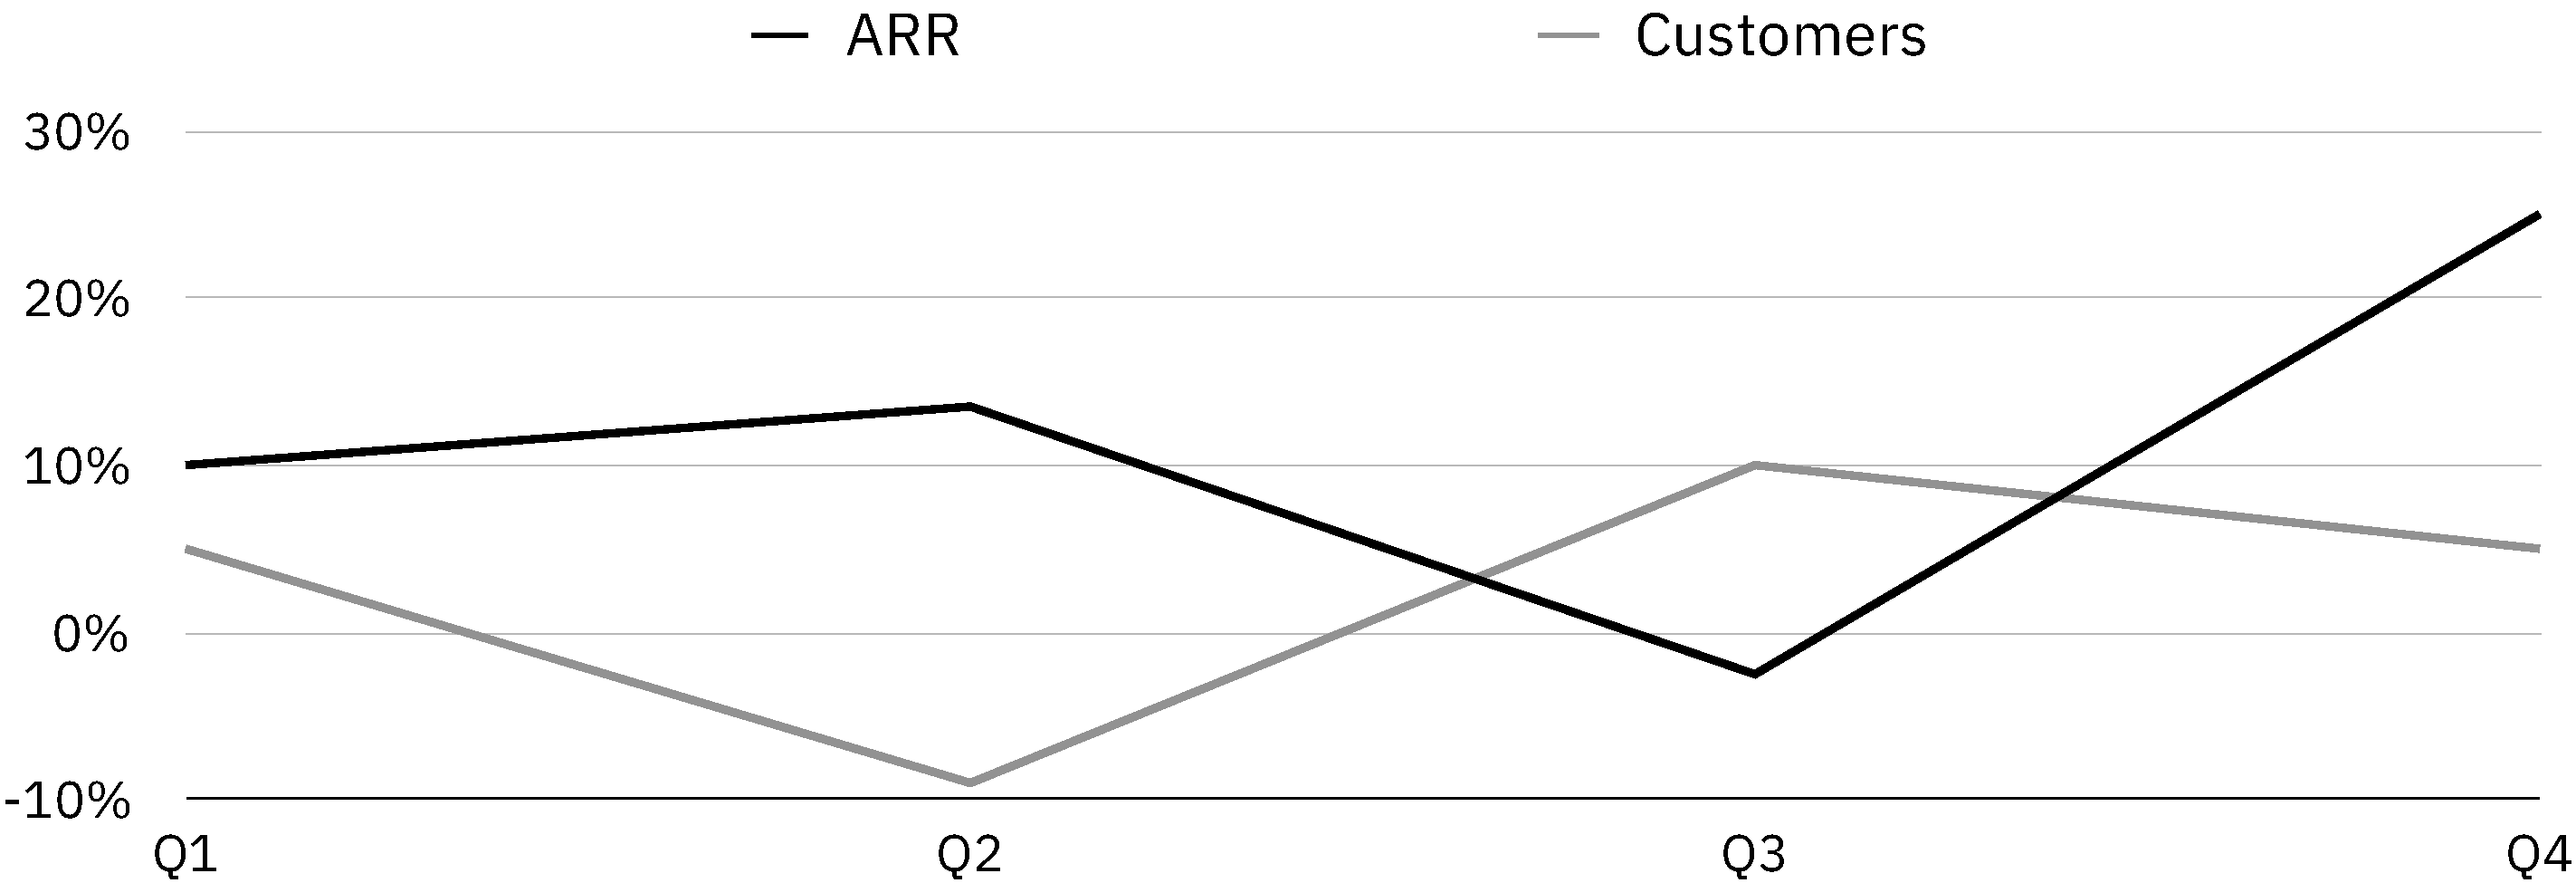
\includegraphics[width=\linewidth]{./include/ARR.pdf}
	\caption{Text block figure caption.}
	\label{fig:example} % Label for referencing this figure in the text automatically
\end{figure}

%------------------------------------------------

\begin{figure*} % Use the figure* environment for full width figures
	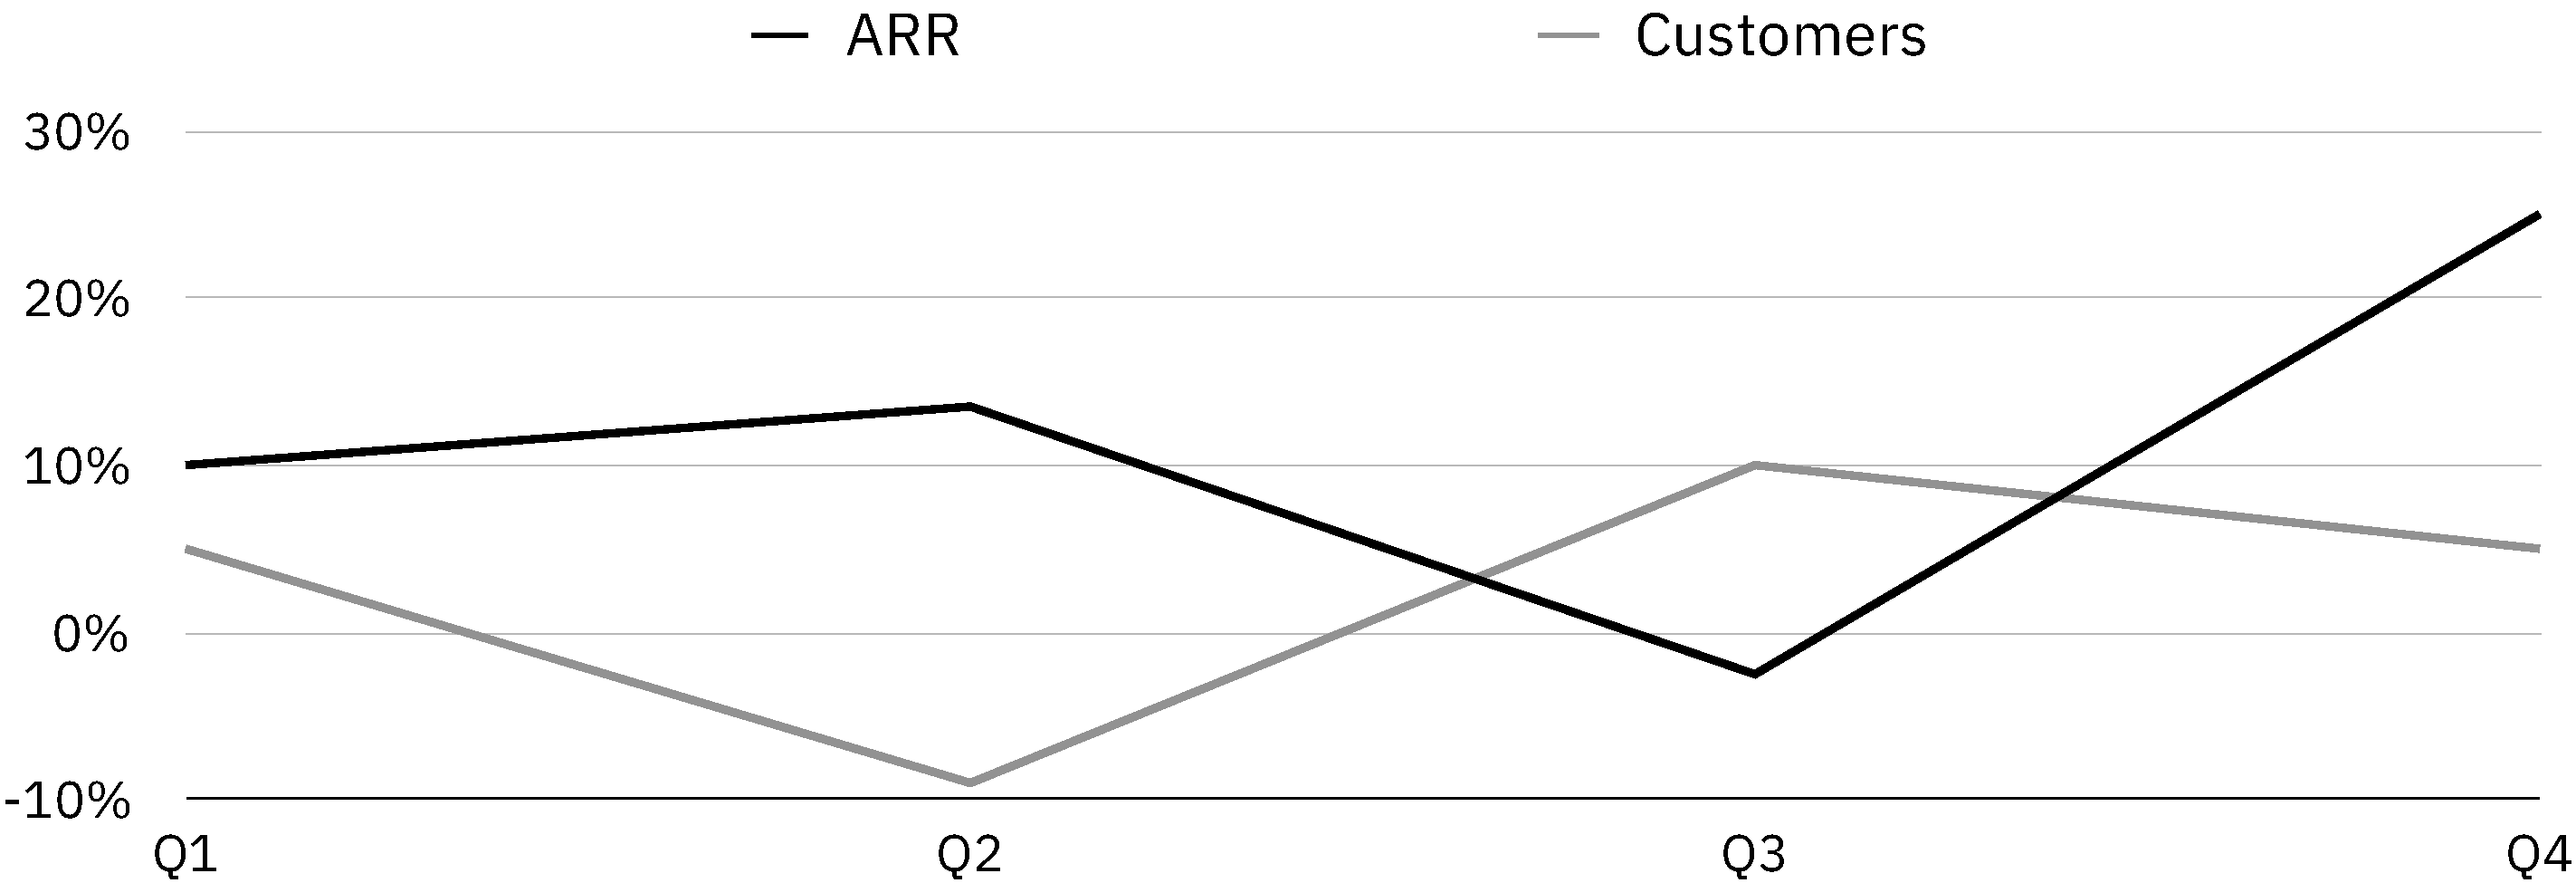
\includegraphics[width=\linewidth]{./include/ARR.pdf}
	\caption{Full width figure caption.}
\end{figure*}

%----------------------------------------------------------------------------------------
%	LISTS
%----------------------------------------------------------------------------------------

\section{List Examples}

\subsection{Bullet Point List}

\nonumsidenote{Bullet point lists can also be created in the margin. For these, we can remove the usual left margin to increase the available horizontal space:\\\medskip \begin{itemize}[leftmargin=*]\item Bullet item one. \item Bullet item two. \item Bullet item three.\end{itemize}}Lorem ipsum dolor sit amet, consectetur adipiscing elit. Praesent porttitor arcu luctus, imperdiet urna iaculis, mattis eros. Pellentesque iaculis odio vel nisl ullamcorper, nec faucibus ipsum molestie. Sed dictum nisl non aliquet porttitor.

\begin{itemize}
	\item First bullet point item
	\begin{itemize}
		\item First indented bullet point item
		\item Second indented bullet point item
		\begin{itemize}
			\item First second-level indented bullet point item
			\item Second second-level indented bullet point item
		\end{itemize}
		\item Third indented bullet point item
	\end{itemize}
	\item Second bullet point item
	\item Third bullet point item
\end{itemize}

Etiam vulputate arcu dignissim, finibus sem et, viverra nisl. Aenean luctus congue massa, ut laoreet metus ornare in. Nunc fermentum nisi imperdiet lectus tincidunt vestibulum at ac elit. Nulla mattis nisl eu malesuada suscipit.

%------------------------------------------------

\subsection{Numbered List}

\nonumsidenote[-2.5cm]{Numbered lists can also be created in the margin. For these, we can remove the usual left margin to increase the available horizontal space:\\\medskip \begin{enumerate}[leftmargin=*]\item Numbered item one. \item Numbered item two. \item Numbered item three.\end{enumerate}}Lorem ipsum dolor sit amet, consectetur adipiscing elit. Praesent porttitor arcu luctus, imperdiet urna iaculis, mattis eros. Pellentesque iaculis odio vel nisl ullamcorper, nec faucibus ipsum molestie. Sed dictum nisl non aliquet porttitor.

\begin{enumerate}
	\item First numbered item
	\begin{enumerate}
		\item First indented numbered item
		\item Second indented numbered item
		\begin{enumerate}
			\item First second-level indented numbered item
			\item Second second-level indented numbered item
		\end{enumerate}
		\item Third indented numbered item
	\end{enumerate}
	\item Second numbered item
	\item Third numbered item
\end{enumerate}

Etiam vulputate arcu dignissim, finibus sem et, viverra nisl. Aenean luctus congue massa, ut laoreet metus ornare in. Nunc fermentum nisi imperdiet lectus tincidunt vestibulum at ac elit. Nulla mattis nisl eu malesuada suscipit.

%------------------------------------------------

\subsection{Description List}

\nonumsidenote{Description lists can also be created in the margin:\\\medskip \begin{description}\item[A1] Description item one. \item[B1] Description item two. \item[C1] Description item three.\end{description}}Lorem ipsum dolor sit amet, consectetur adipiscing elit. Praesent porttitor arcu luctus, imperdiet urna iaculis, mattis eros. Pellentesque iaculis odio vel nisl ullamcorper, nec faucibus ipsum molestie. Sed dictum nisl non aliquet porttitor.

\begin{description}
	\item[Item One] Lorem ipsum dolor sit amet, consectetur adipiscing elit. Praesent porttitor arcu luctus, imperdiet urna iaculis, mattis eros. Pellentesque iaculis odio vel nisl ullamcorper, nec faucibus ipsum molestie.
	\item[Item Two] Sed dictum nisl non aliquet porttitor.
	\begin{description}
		\item[Subitem] Maecenas consectetur metus at tellus finibus condimentum. Proin arcu lectus, ultrices non tincidunt et, tincidunt ut quam. Integer luctus posuere est, non maximus ante dignissim quis.
		\begin{description}
			\item[Subsubitem] Maecenas consectetur metus at tellus finibus condimentum. Proin arcu lectus, ultrices non tincidunt et, tincidunt ut quam. Integer luctus posuere est, non maximus ante dignissim quis.
	\end{description}
	\end{description}
	\item[Item Three] Etiam vulputate arcu dignissim, finibus sem et, viverra nisl. Aenean luctus congue massa, ut laoreet metus ornare in. Nunc fermentum nisi imperdiet lectus tincidunt vestibulum at ac elit. Nulla mattis nisl eu malesuada suscipit.
\end{description}

Etiam vulputate arcu dignissim, finibus sem et, viverra nisl. Aenean luctus congue massa, ut laoreet metus ornare in.

%----------------------------------------------------------------------------------------
%	REFERENCING CITATIONS
%----------------------------------------------------------------------------------------

\section{Referencing Citations}

This statement requires citation \autocite{Smith:2024jd}.

This statement requires multiple citations \autocite{Smith:2024jd, Smith:2023qr}.

This short citation is in the margin\sidecite{Smith:2023qr}.

This long citation is in the margin\fullsidecite{Smith:2024jd}.

This statement has an in-text citation: \textcite{Smith:2024jd}.

%----------------------------------------------------------------------------------------
%	LINKS
%----------------------------------------------------------------------------------------

\section{Link Examples}

This is a URL link: \href{https://www.duckduckgo.com}{DuckDuckGo}.\nonumsidenote{Links can be clicked in the PDF to navigate to the linked website or email address.}

This is a email link: \href{mailto:example@example.com}{example@example.com}.

This is a monospaced URL link: \url{https://duckduckgo.com}.


%----------------------------------------------------------------------------------------
%	CODE
%----------------------------------------------------------------------------------------

\section{Displaying Code}

The block below is a code listing. It displays code in an easy to use way with line numbers for quick reference to specific parts of the code.

\begin{lstlisting}
{
	"city": [
		{
			"id": 1,
			"name": "Toronto",
			"country": "Canada",
			"population": 6200000
		},
		{
			"id": 2,
			"name": "New York",
			"country": "United States of America",
			"population": 8800000
		}
	]
}
\end{lstlisting}

%----------------------------------------------------------------------------------------
%	 REFERENCES/BIBLIOGRAPHY
%----------------------------------------------------------------------------------------

\newpage

\addcontentsline{toc}{section}{Reference List} % Add the bibliography to the table of contents

\begin{twothirdswidth} % Content in this environment to be at two-thirds of the whole page width
	\printbibliography[title=Reference List] % Output the bibliography with a custom section title
\end{twothirdswidth}

%----------------------------------------------------------------------------------------
%	APPENDICES
%----------------------------------------------------------------------------------------

\newpage

\section*{Appendices}

\begin{appendices}

\section{Appendix Section}

Lorem ipsum dolor sit amet, consectetur adipiscing elit. Aliquam auctor mi risus, quis tempor libero hendrerit at. Duis hendrerit placerat quam et semper. Nam ultricies metus vehicula arcu viverra, vel ullamcorper justo elementum. Pellentesque vel mi ac lectus cursus posuere et nec ex. Fusce quis mauris egestas lacus commodo venenatis. Ut at arcu lectus. Donec et urna nunc. Morbi eu nisl cursus sapien eleifend tincidunt quis quis est. Donec ut orci ex. Praesent ligula enim, ullamcorper non lorem a, ultrices volutpat dolor. Nullam at imperdiet urna. Pellentesque nec velit eget euismod pretium.

\section{Appendix Section}

Lorem ipsum dolor sit amet, consectetur adipiscing elit. Aliquam auctor mi risus, quis tempor libero hendrerit at. Duis hendrerit placerat quam et semper. Nam ultricies metus vehicula arcu viverra, vel ullamcorper justo elementum. Pellentesque vel mi ac lectus cursus posuere et nec ex. Fusce quis mauris egestas lacus commodo venenatis. Ut at arcu lectus. Donec et urna nunc. Morbi eu nisl cursus sapien eleifend tincidunt quis quis est. Donec ut orci ex. Praesent ligula enim, ullamcorper non lorem a, ultrices volutpat dolor. Nullam at imperdiet urna. Pellentesque nec velit eget euismod pretium.

\section{Appendix Section}

Lorem ipsum dolor sit amet, consectetur adipiscing elit. Aliquam auctor mi risus, quis tempor libero hendrerit at. Duis hendrerit placerat quam et semper. Nam ultricies metus vehicula arcu viverra, vel ullamcorper justo elementum. Pellentesque vel mi ac lectus cursus posuere et nec ex. Fusce quis mauris egestas lacus commodo venenatis. Ut at arcu lectus. Donec et urna nunc. Morbi eu nisl cursus sapien eleifend tincidunt quis quis est. Donec ut orci ex. Praesent ligula enim, ullamcorper non lorem a, ultrices volutpat dolor. Nullam at imperdiet urna. Pellentesque nec velit eget euismod pretium.

\end{appendices}

%----------------------------------------------------------------------------------------

\end{document}
